 
 
\chapter{Fourier transform with values in a finite field}
\label{chap-extension-finite-field-values}
 
 
We have already encountered finite fields many times, in particular in chapter \oldref{chap-applications-trans-fourier-grpe-finite}. However, we limited ourselves to exploiting them as \textit{start} domains of the functions we wanted to analyze. However, it is very common to manipulate data with values in a finite set, which we can often provide with a finite field structure. The most striking example is binary data, which can be modeled by functions with values in $ \FF_2 \simeq \{0, \, 1\} $. In this chapter, we will present many similar situations, and we will see how Fourier tools naturally extend to such field structures.
 
% ------------------------------------------------- -----
% ------------------------------------------------- -----
% ------------------------------------------------- -----
% section - Calculations on a finite field                           
% ------------------------------------------------- -----
% ------------------------------------------------- -----
% ------------------------------------------------- -----
\section{Finite field calculations}
% \addcontentsline{toc}{section}{Finite field calculations}
\label{sect1-calculations-finite-field}
 
 
Since the beginning of the talk, we have limited ourselves to the study of functions with values in the field $ \CC $ of the complexes, and we are particularly interested in the morphisms of $ G $ (abelian finite group) in the group multiplicative $ \CC^* $. However, most of the results remain valid if we consider the morphisms of $ G $ in any commutative field. In this section, we will take a closer look at the case of finite fields. Not only will we take the results already stated in the previous chapters, but we will particularize them and explain why and how to perform the calculations in a finite field.
 
 
It is a question of carrying out our calculations modulo a prime number $ p $. We must be careful not to believe that we are going to restrict ourselves to the only field $ \FF_p \eqdef \ZZ/p \ZZ $. For example, in Paragraph~\ref{sect2-trans-cyclotomic-field}, we are going to place ourselves in a larger field, of the type $ \FF_{p^r} $, where $ r \geq 1 $, to define a transform of arbitrary length.
% ------------------------------------------------- -----
% ------------------------------------------------- -----
% sub-section - Fourier transform on a finite field                           
% ------------------------------------------------- -----
% ------------------------------------------------- -----
\subsection{Fourier transform on a finite field}
\label{sect2-trans-fourier-finite-field}
 
 
\index{Finite field} We therefore fix a prime integer $ p $. All our calculations will be carried out modulo $ p $. To construct a valued transform in a finite field, we need a \textit{primitive root} \ordin{n}{th} of unity. Let's clarify what this means.
 
\begin{defn}[Primitive root]
\index{Root!of unit} \index{Root!primitive} Let $ K $ be a field. An element $ \zeta \in K $ is called \textit{root of unit} if it is a finite order element of $ K^* $, that is, if there is an integer $ s> 0 $ such that $ \zeta^s = 1 $. \\An element of order $ n $ of $ K^* $ is called primitive root \ordin{n}{th} of the unit, this which means that $ \zeta^{n} = 1 $ and that for any $ s $ such that $ 0 <s <n $, we have $ \zeta^{s} \neq 1 $.
\end{defn}
In a finite field $ K $ of cardinal $ q = p^r $, any element of $ K^* $ is necessarily a root \ordin{(q-1)}{th} of the unit. Of course, the existence of a root \ordin{n}{th}, for any $ n $, is not assured. Indeed, the order of any element of $ K^* $ is a divisor of $ q-1 $. Conversely, if $ n | q-1 $, i.e. $ -1 = nk $, then, if we denote by $ \omega $ a generator of $ K^* $, $ \zeta = \omega^{k} $ is a primitive \ordin{n}{th} root.
 
 
For simplicity, we'll assume that $ q = p $ is a prime number. We also admit that we have $ \zeta $, a \ordin{n}{th} primitive root of the unit over $ \FF_p $. It is then very simple to define the Fourier transform with values in the field $ \FF_p $.
 
\begin{defn}[Transform over $ \FF_p $]
For a vector $ f \in (\FF_p)^n $, we define the Fourier transform:
\begin{equation}
\label{eq-defn-transforme-fp}
\forall j \in \{0, \ldots, \, n-1\}, \quad \Ff(f) [j] = \wh{f}[j] \eqdef \sum_{k = 0}^{n-1}{f [k] \zeta^{- kj}}.
\end{equation}
\end{defn}
The Fourier transform on $ \FF_p $ has exactly the same properties as the classical Fourier transform; here they are briefly recalled.
 
\begin{prop}[Properties]
\label{prop-prtes-tfd-finite-field}
$ \Ff $ is an algebra isomorphism from $ ((\FF_p)^n, \, *) $ to $ ((\FF_p)^n, \, \cdot) $, where we denote $ * $ the product of circular convolution and $ \cdot $ the product component by component. Its inverse is given by
\begin{equation}
\label{eq-defn-tfd-finite-field}
\Ff^{-1} (f) [n] = n^{-1} \sum_{k = 0}^{n-1}{f [k] \zeta^{kn}}.
\end{equation}
\end{prop}
 
 
 
\index{Product!of integers} The Fourier transform modulo $ p $ has a definite advantage: all the calculations are done with integers (certainly modulo $ p $, but in the end, we always carry out additions and multiplications of integers). There is thus no numerical error likely to taint the results of calculations. On the other hand, in calculations requiring high precision, the use of a conventional FFT can lead to errors. When, for example, we want to calculate the product of two large integers (using the technique presented in Paragraph~\ref{sect2-multiplication-integers}), it is very important to minimize the numerical errors, since we want, at final, find whole values (we are actually going to round to the nearest whole number). For example, in \cite{bailey-pi}, the author explains that in double precision, past 10 million decimal places, the FFT algorithm, used for calculations of integer products, gave bad results because of rounding errors. This is why algorithms for calculations on finite fields (and more generally on $ \ZZ/m \ZZ $) are at the heart of computer systems requiring high precision integer calculations.
 
 
Beyond all these advantages, we must keep in mind that the result obtained by transforming on a finite field no longer has any meaning \guill{physics}. Indeed, the Fourier transform with values in $ \CC $ represents an approximation of the continuous Fourier transform on $ \RR $, which is of course far from being the case for the transform on a finite field. We can consider the transformation performed in complexes as a means of passing from a temporal representation of the data to a frequency representation, whereas there is no such obvious interpretation for the transformation carried out on $ \FF_p $.

% ------------------------------------------------- -----
% ------------------------------------------------- -----
% sub-section - A special case                           
% ------------------------------------------------- -----
% ------------------------------------------------- -----
\subsection{A special case}
\label{sect2-a-particular-case}
 
 
The problem we face in building this transform is finding a primitive \ordin{n}{th} root of unity. To fully understand the difficulties that we encounter, let's start by showing a case where everything goes well, but which, as we will see, is very restrictive.
 
 
We assume that we have chosen $ n = p-1 $. We know that the multiplicative group $ \FF_p^* = \FF_p - \{0\} $ is a finite cyclic group. Consequently, it has a generator element: let us denote the $ \zeta $. By definition, we therefore have
\begin{equation*}
\FF_p^* = \{1, \, \zeta, \, \zeta^2, \ldots, \, \zeta^{n-1}\} \quad \text{and} \zeta^n = 1.
\end{equation*}
We have therefore exhibited a primitive \ordin{n}{th} root of unity, but at the cost of a particular choice for the value of $ n $. A naive algorithm to determine a generator of the multiplicative group $ (\ZZ/n \ZZ)^* $ consists in trying all the elements of the group one by one. A more efficient algorithm is presented in the book by \nompropre{Cohen} \cite{cohen-computational}.
% ------------------------------------------------- -----
% ------------------------------------------------- -----
% sub-section - Cyclotomic bodies                           
% ------------------------------------------------- -----
% ------------------------------------------------- -----
\subsection{Cyclotomic bodies}
\label{sect2-cyclotomic-field}
 
 
In the previous paragraph, we built a Fourier transform of size $ n $ on $ \FF_p $ in a very specific case, which imposed a relation between the integers $ n $ and $ p $. However, one may wish to choose these two parameters independently, for example in the frequent case where one wishes to produce DFTs of very large size, much more than $ p $. The problem is that there is no reason for the field $ \FF_p \eqdef \ZZ/p \ZZ $ to contain primitive \ordin{n}{th} roots. We are therefore going to have to work in an extension of $ \FF_p $, that is to say a certain $ \FF_{p^r} $ for $ r \in \NN^* $.
 
 
To carry out the search for this extension, we need to study the irreducible factors of the polynomial $ X^n-1 $, since these will be the minimal polynomials of a possible primitive root. Let us recall without demonstrating what these irreducible factors are on the field $ \QQ $.
 
\begin{thmdefn}[Cyclotomic polynomials]
 
\index{Polynomial!cyclotomic} \label{notation-64} We denote by $ \Phi_n $ the \ordin{n}{ième} cyclotomic polynomial, defined as follows:
\begin{equation*}
\Phi_n (X) \eqdef \prod_{k \in (\ZZ/n \ZZ)^*} \left(X- e^{\frac{2 \imath \pi k}{n}} \right).
\end{equation*}
Cyclotomic polynomials verify
\begin{equation}
\label{eq-decomposition-xn-1}
X^n-1 = \prod_{d | n}{\Phi_d (X)}.
\end{equation}
They have coefficients in $ \ZZ $, and moreover, they are irreducible in $ \QQ [X] $.
\end{thmdefn}
For a proof of this theorem, as well as a very clear construction of finite fields, we can look at the book of \nompropre{Demazure} \cite{demazure}.
 
\begin{exmp}
The equation \eqref{eq-decomposition-xn-1} provides an algorithm which allows to determine by induction the cyclotomic polynomials, of which here are some examples:
\begin{equation*}
\begin{split}
\Phi_1 (X) & = X - 1, \\
\Phi_2 (X) & = X + 1, \\
\Phi_3 (X) & = X^2 + X + 1, \\
\Phi_6 (X) & = X^2 - X - 1.
\end{split}
\end{equation*}
\index{Maple@\Maple{}} The \Maple{} \ref{listing-calculus-cyclotomic-polynomials} program calculates a cyclotomic polynomial. For more on this, see the exercise \oldref{exo-calculus-pol-cyclotomic}.
 
\begin{listing} \begin{footnotesize}
{\upshape
\begin{tabular}{l}
\texttt{\pwith{}(numtheory): cyclotomic(105, X);} \\
\texttt{$ 1 + X - X^{8} + X^{2} - X^{5} - 2 \, X^{7} + X^{35} - X^{28} + X^{48 } + X^{46} - X^{43} - 2 \, X^{41} - X^{40} - X^{39} + X^{36} + X^{34} $} \\\texttt{$ \mbox{} + X^{33} + X^{31} - X^{26} - X^{24} - X^{22} - X^{20} + X^{17} + X^{16} + X^{15} + X^{14} + X^{12} - X^{9} - X^{6} + X^{47} $} \\\texttt{$ \mbox{} - X^{42} + X^{32} + X^{13} $} \\
\end{tabular}
}
\end{footnotesize}
\caption{Computing a cyclotomic polynomial}
\label{listing-calculus-cyclotomic-polynomials}
\end{listing}
 
\end{exmp}
 
 
 
The polynomials $ \Phi_n $ being with coefficients in $ \ZZ $, we can therefore reduce them modulo $ p $ and regard them as elements of $ \FF_p [X] $. Although they are irreducible on $ \QQ $, there is no reason why they are still irreducible on $ \FF_p $. More precisely, it is the following theorem which will allow us to construct the extension of fields which we need.
 
\begin{prop}[Cyclotomy on $ \FF_p $]
\label{prop-cyclotomy-fp}
We assume $ \PGCD (n, \, p) = 1 $. Let $ r $ be the order of $ p $ in the group $ (\ZZ/n \ZZ)^* $, i.e. the smallest integer $ t $ such that $ p^t = 1 $ modulo $ n $. Then the cyclotomic polynomial $ \Phi_n (X) $ decomposes in $ \FF_p [X] $ into the product of irreducible polynomials of degree $ r $, all different.
\end{prop}
\begin{proof}
Since $ n $ is prime with $ p $, the polynomial $ X^n-1 $ is prime with its derivative $ n X^{n-1} $, so it does not have a multiple root in an extension. With the relation \eqref{eq-decomposition-xn-1}, we therefore deduce that the polynomial $ \Phi_n $ has no multiple factor. It is therefore sufficient to show that any irreducible factor of $ \Phi_n $ is of degree $ r $. \\Let $ P $ be an irreducible factor of degree $ s $. We denote by $ K = F_p [X] / (P) $ the residual field. Its cardinality is $ | K | = p^s $. The image $ \zeta $ of the undetermined $ X $ in $ K $ is a primitive root of unity, since $ P $ is an irreducible factor of $ X^n-1 $ and $ \zeta $ is root of $ P $. Since every element $ x $ of $ K^* $ satisfies $ x^{p^s-1} = 1 $, in particular, $ \zeta^{p^s-1} = 1 $, and the definition of a primitive root \ordin{n}{th} implies that $ n | p^s-$ 1. By definition of the order $ r $ of $ p $ in $ (\ZZ/n \ZZ)^* $, we therefore have $ r \leq s $. \\Let us show the inverse inequality. Like $ n | p^r - 1 $, we have $ p^r - 1 = \lambda n $, hence $ \zeta^{p^r - 1} = (\zeta^n)^{\lambda} = 1 $ , so $ \zeta^{p^r} = \zeta $. Let $ k $ denote the subfield of $ K $ formed by the roots of the equation $ X^{p^r} = X $. It contains $ \zeta $ which generates $ K^* $, so it is actually equal to $ K $ integer. Since $ X^{p^r} - X $ has at most $ p^r $ distinct roots, we get that $ | K | = | k | \leq p^r $, so $ s \leq r $ which is the inequality sought.
\end{proof}
 
 
\begin{rem}
\label{rmk-cyclotomy-cas-special}
In the case where the integers $ n $ and $ p $ are not prime to each other, $ n $ is a multiple of $ p $, that is $ n = mp^t $, where this time $ m $ is prime with $ p $. We then write
\begin{equation*}
X^n - 1 = (X^m)^{p^t} - 1^{p^t} = (X^m - 1)^{p^t}.
\end{equation*}
We can now apply the previous proposition to the polynomial $ X^m - 1 $ to find a decomposition of $ X^n-1 $.
\end{rem}
 
 
\begin{rem}
In fact, the proposition \ref{prop-cyclotomy-fp} is still valid on a field of the type $ \FF_q $ where $ q = p^t $ (without modification of the proof). The polynomial $ \Phi_n $ decomposes in $ \FF_q [X] $ into a product of irreducible polynomials of degree $ r $, where $ r $ is the order of $ q $ in $ (\ZZ/n \ZZ)^* $. We must be careful: looking at the polynomial $ \Phi_n $ on $ \FF_p $ amounts to reducing its modulo $ p $ coefficients (and not modulo $ q $!). However, since there are more elements in $ \FF_q $ than in $ \FF_p $, it is possible that some irreducible factors of $ \Phi_n $ on $ \FF_p $ decompose on $ \FF_q $.
\end{rem}
 
 
 
If we denote by $ P $ an irreducible factor of $ \Phi_n $, the field $ K \eqdef \FF_p [X] / (P) $ is therefore the extension of $ \FF_p $ that we are looking for. It is a field of cardinal $ p^r $, and we can see it as a vector space of dimension $ r $ on $ \FF_p $, simply by considering its elements as polynomials of degree at most $ r-1 $ . We generally write $ \FF_{p^r} $ this field, but it should not be confused with $ \ZZ/p^r \ZZ $: in fact, in $ K $, we continue to perform the modulo addition $ p $, and the multiplication is more complex since it corresponds to the multiplication of the polynomials modulo $ P $. Finally, let us note that we have thus found a primitive root of unity. It suffices to consider the class of the indeterminate $ X $ in $ K $: it is in fact a root that we will denote by $ \zeta $ of $ P $ in $ K $. We can then see the field $ K $ as $ \FF_p [\zeta] $, the field generated by $ \zeta $ on $ \FF_p $. We name this field the \textit{cyclotomic field of index $ n $} on $ \FF_p $.
 
\begin{exmp}
\index{Quotient} If we consider the polynomial
\begin{equation*}
\Phi_{15} (X) = 1 - X + X^3 - X^4 + X^5 - X^7 + X^8 \in \ZZ [X].
\end{equation*}
Since the order of 2 in $ (\ZZ/15 \ZZ)^* $ is 4, $ \Phi_{15} $ decomposes over $ \FF_2 $ as a product of 2 irreducible degree 4 polynomials:
\begin{equation*}
\Phi_{15} (X) = (1 + X + X^4) (1 + X^3 + X^4) \; \in \FF_2 [X].
\end{equation*}
A decomposition field of $ \Phi_{15} $ is therefore for example
\begin{equation*}
\FF_2 [X] / (1 + X + X^4) \simeq \FF_{2^4} \simeq \FF_2 [\alpha],
\end{equation*}
where we denote by $ \alpha $ a root of $ 1 + X + X^4 $ (i.e. the class of the indeterminate $ X $ in the quotient field $ \FF_2 [X] / ( 1 + X + X^4) $).
\end{exmp}
 
 
 
In a practical way, to build this field, it is first necessary to calculate the polynomial $ \Phi_n $ (for example by using by induction the relation \eqref{eq-decomposition-xn-1}), then to find a factor irreducible from $ \Phi_n $ to $ \FF_p $. To do this, we can use \Maple{}, the whole process being detailed in the first program of paragraph \annexeref{sect1-listing-transform-finite-body}. An algorithm allowing to factorize polynomials over a finite field is the \textit{Berlekamp} algorithm. It is detailed in the book of \nompropre{Demazure} \cite{demazure}. \index{Berlekamp@\nompropreindex{Berlekamp}} \index{Algorithme!De Berlekamp}


% ------------------------------------------------- -----
% ------------------------------------------------- -----
% sub-section - Transform on a cyclotomic field                           
% ------------------------------------------------- -----
% ------------------------------------------------- -----
\subsection{Transform on a cyclotomic field}
\label{sect2-trans-cyclotomic-field}
 
 
Thanks to the decomposition of the polynomial $ \Phi_n $ over the field $ \FF_p $, we succeeded in constructing an extension of $ \FF_p $, denoted $ K \eqdef \FF_{p^r} $, in which there is a root \ordin{n}{th} primitive of the unit, $ \alpha $. In addition, knowing its minimal polynomial $ P $ allows us to calculate with the elements of $ K $ (which are vectors of $ r $ elements of $ \FF_p $), since it suffices to use the polynomial multiplication modulo $ P $.
 
 
By placing ourselves in the field $ K $, we therefore define the transform of a vector $ f \in K^n $ by the equation \eqref{eq-defn-transforme-fp}. This time, $ \Ff(f) $ is also a vector of $ K^n $. In practice, we often use this transform for data which are elements of $ (\FF_p)^n $, but of course we must keep in mind that the result has no reason to stay in $ \FF_p $. We find the same phenomenon as for the computation of the (classical) DFT of a real vector, for which we are obliged to place ourselves in the $ \CC $ extension of the field of real numbers. Recall that if we denote the elements of $ \FF_{p^r} $ as vectors (rather than polynomials), an element of the base field $ \FF_p $ is distinguished by the fact that only the first component of the vector is not zero.
 
 
This construction of a fast transform algorithm for an arbitrary length $ N $ will be used in Section~\ref{sect1-applications-correctors-codes}. It will in fact be a question of decoding certain corrective codes using the Fourier transform. We will see that the use of a super-field (which may seem a little artificial for the moment) then becomes very natural to find the set of codes verifying certain properties (we call them \textit{cyclic codes}).

% ------------------------------------------------- -----
% ------------------------------------------------- -----
% sub-section - Effective calculations                           
% ------------------------------------------------- -----
% ------------------------------------------------- -----
\subsection{Effective calculations}
\label{sect2-effective-calculations}
 
 
We will be able to use the Fourier transform with values in a finite field to do convolution calculations. As all the calculations are carried out modulo $ p $, we will have to choose an integer $ p $ large enough to be able to retrieve results of calculations in $ \ZZ $, and not modulo $ p $.
 
 
The best example of the use of this Fourier transform is the computation of products of large integers, written in base $ b $. The paragraph \ref{sect2-multiplication-integers}, explains how to calculate the product of two integers using an acyclic convolution. We can easily determine a bound on the value of the inputs of a linear convolution of two integers represented in base $ b $:
\begin{equation*}
| f \star g [k] | = \left| \sum_{l = 0}^{n-1}{f [l] g [kl]} \right| \leq \sum_{l = 0}^{n-1}{| f [l] | | g [kl] |} \leq n (b-1)^2.
\end{equation*}
In order to be able to calculate exactly the product of two integers, $ | f \star g [k] | <p $. We will therefore be interested in choosing $ p> n (b-1)^2 $.
 
 
\index{FFT} \index{Dichotomy} To finish, it is necessary to say a few words about the practical implementation of the algorithm for calculating the transform. Most often, we will consider that $ n $ is of the form $ 2^k $, and we will use the dichotomous FFT algorithm presented in Section~\ref{sect1-transform-fast}. The details of the algorithm remain unchanged. Among other things, if $ \zeta $ is the root of order $ 2^k $ sought, then $ \zeta^2 $ will be the root of order $ 2^{k-1} $, etc. Of course, it is necessary to replace the operations in the field of the complexes by operations in the finite field $ K = \FF_{p^r} $. We must therefore choose a way to represent the elements of the field $ K $, and know how to multiply them. If we have looked for the primitive root $ \zeta $ as indicated in Paragraph~\ref{sect2-cyclotomic-field}, we have a very natural way of doing it. Indeed, we have at the same time the minimal polynomial $ P $ of $ \zeta $, of degree $ r $, and we can therefore represent the elements of the field as polynomials of degree at most $ r-1 $ (c'that is, by vectors of size $ r $ in the computer memory). The addition is then carried out component by component, while the multiplication is carried out as a multiplication of polynomials modulo $ P $. This multiplication is calculated in the classic way, then by taking the remainder of the Euclidean division by $ P $.
 
 
The \listingterme{} \Maple{} of the \ref{sect1-listing-transform-finite-body} section, performs step by step the different steps leading to the construction of a transform on a finite field. It starts with the factorization of $ \Phi_n $ on $ \FF_p $, and contains a recursive FFT algorithm. It makes full use of the \Maple{} facilities, which eliminates the need to worry about operations in the field $ \FF_{p^r} $. Finally, it will be noted that it precedes the program on \textit{corrective codes BCH} (paragraph \ref{sect1-listing-decoding-bch}), the latter using the procedures for calculating transforms on a finite field.

% ------------------------------------------------- -----
% ------------------------------------------------- -----
% ------------------------------------------------- -----
% section - Calculations on a ring                           
% ------------------------------------------------- -----
% ------------------------------------------------- -----
% ------------------------------------------------- -----
\section{Calculations on a ring}
% \addcontentsline{toc}{section}{Calculations on a ring}
\label{sect1-calculations-ring}
 
\index{Ring} It is natural, after having presented the Fourier transform with values in a finite field, to try to extend this notion to any commutative ring. This generalization is not at all free, since it will make it possible to calculate in any ring $ \ZZ/m \ZZ $ at a lower cost (the calculation of sums and products is done quite simply modulo $ m $). We will thus obtain an FFT algorithm much simpler than the one built in the previous paragraph, which required the passage in an over-field and the computation of Euclidean divisions to perform the products in this field. Of course, just like in the simplistic example of Paragraph~\ref{sect2-a-particular-case}, where we had $ n = p-1 $, we will once again have limitations on the choice of $ n $ or $ p $. However, we will see that by considering rings of the type $ \ZZ/2^r \ZZ $, we can build a very simple FFT algorithm, where the primitive root search becomes trivial.
% ------------------------------------------------- -----
% ------------------------------------------------- -----
% sub-section - Main roots of the unit                           
% ------------------------------------------------- -----
% ------------------------------------------------- -----
\subsection{Main roots of the unit}
\label{sect2-main-roots}
 
In this section, we consider more general structures, namely arbitrary commutative rings. In practice, we mainly use the ring $ \ZZ/m \ZZ $, where $ m $ is a positive integer, which allows calculations to be done in a simple way using a computer (addition and multiplication modulo $ m $). A problem arises when one wishes to define a Fourier transform using the equation \eqref{eq-defn-tfd-finite-field} on any ring $ A $: the transformation thus defined does not have no reason to be bijective. This is due to the presence of divisors of zero in the ring $ A $. Recall that a divisor of zero $ x \neq 0 $, is an element of $ A $ such that there exists a $ y \neq 0 $ verifying $ xy = 0 $. For example, in the ring $ \ZZ/6 \ZZ $, we have the equality $ 2 \cdot 3 = 0 $, so the elements $ 2 $ and $ 3 $ are divisors of zero. To overcome this problem, we will have to impose additional restrictions on the choice of the root \ordin{n}{ième} $ \zeta $. By following the notations of \nompropre{Demazure} \cite{demazure}, we will introduce the concept of \textit{main root of the unit}.
 
\begin{defn}[Main root of unit]
\index{Main!root of unit} \index{Divisor of zero} Let $ A $ be any commutative ring. An element $ \zeta \in A $ is called the main \ordin{n}{th} root of the unit if: \begin{itemize}
\item [{\upshape (i)}] we have $ \zeta^n = 1 $ (in particular, $ \zeta $ is invertible).
\item [{\upshape (ii)}] for any $ i \in \{1, \ldots, \, n-1\} $, the element $ 1 - \zeta^i $ is not a divisor of zero in $ A $. This means that if $ a \zeta^i = a $, then $ a = 0 $.
\end{itemize}
\end{defn}
 
 
\begin{rem}
\index{Ring!integrates} The fact that $ \zeta^i-1 $ is not a divisor of zero for $ i = 1, \ldots, \, n-1 $ implies in particular that $ \zeta^i \neq $ 1, so a principal root is a primitive root. We see that if the ring is integral (and a fortiori if it is a field), the notions of primitive \ordin{n}{ième} root and of main \ordin{n}{ième} root coincide. On the other hand, if we consider for example the ring $ \ZZ/15 \ZZ $, we see that the element $ 2 $ is a primitive root \ordin{4}{ième} of the unit, but it is not not principal, since $ 2^2-1 = $ 3 is a divisor of zero.
\end{rem}
We are therefore going to find a main root of the unit, for example by carrying out an exhaustive search among the elements of $ A^* $. As this calculation is done once and for all, it is not important to have a fast algorithm. We can then define the discrete Fourier transform with values in $ A $ in the usual way.
 
\begin{defn}[Fourier transform in a ring]
Let $ A $ be a commutative ring, and $ \zeta \in A^* $ a main \ordin{n}{th} root. For a vector $ f \in A^n $, we define the Fourier transform $ \Ff $ as well as another map denoted $ \wt{\Ff} $ by
\begin{align}
\label{eq-defn-transform-ring}
\forall j \in \{0, \ldots, \, n-1\}, \quad \Ff(f) [j] & \eqdef \sum_{k = 0}^{n-1}{f [k ] \zeta^{- kj}}, \\
\forall j \in \{0, \ldots, \, n-1\}, \quad \wt{\Ff} (f) [j] & \eqdef \sum_{k = 0}^{n-1}{f [k] \zeta^{kj}}.
\end{align}
\end{defn}
In order to study the relations between these two transforms, we need the following lemma.
 
\begin{lem}
\label{lem-transf-fourier-ring}
Let $ A $ be a commutative ring and $ \zeta $ a main \ordin{n}{th} root of unity. We then have
\begin{equation*}
\sum_{i = 0}^{n-1}{\zeta^{ki}} = \left\{\begin{array}{ll} n & \text{si} k = 0 \; \mod{n} \\0 & \text{otherwise} \end{array} \right. .
\end{equation*}
\index{Divisor of zero} Also, $ n $ is not a divisor of zero in the ring.
\end{lem}
\begin{proof}
We will prove the following polynomial equality:
\begin{equation*}
X^n - 1 = \prod_{i = 0}^{n-1}{\left(X- \zeta^i \right)}.
\end{equation*}
Denote by $ P (X) = X^n - 1 $. We have $ P (1) = 0 $, so $ P $ is written $ (X - 1) Q (X) $, where $ Q $ is a unit polynomial (indeed, like the polynomial $ X-1 $ is unitary, we can realize the Euclidean division of $ P $ by $ X-1 $ and see that the remainder is zero). As $ \zeta $ is also the root of $ P $, we see that $ (\zeta - 1) Q (\zeta) = 0 $, and the fact that $ \zeta - 1 $ is not a divisor of zero allows us to conclude that $ Q (\zeta) = 0 $. We start again with $ Q $, which we write in the form $ (X - \zeta) R (X) $. We then have $ P (\zeta^2) = (\zeta^2-1) \zeta (\zeta - 1) R (\zeta^2) $. The fact that $ \zeta^2 - 1 $ is not a divisor of zero allows us to state that $ R (\zeta^2) = 0 $. We continue in this way until finding the announced factorization. By removing the factor $ X - $ 1, we find
\begin{equation*}
X^{n-1} + \cdots + X + 1 = \prod_{i = 1}^{n-1}{\left(X- \zeta^i \right)}.
\end{equation*}
Hence, by evaluating the previous equality in $ X = $ 1,
\begin{equation*}
n 1_A = \prod_{i = 1}^{n-1}{\left(1- \zeta^i \right)}.
\end{equation*}
This shows that $ n $ is not a divisor of zero in $ A $. Evaluating the same equality again, but for $ X = \zeta^k $, we obtain the announced equality.
\end{proof}
We can then state the main result.
 
\begin{thm}[Properties of the transform on a ring]
We denote by $ * $ the product of circular convolution and $ \cdot $ the product component by component. $ \Ff $ is an algebra morphism from $ (A^n, \, *) $ into $ (A^n, \, \cdot) $. We have the connections
\begin{equation*}
\forall f \in A^n, \quad \Ff(\wt{\Ff} (f)) = nf \quad \quad \text{and} \quad \quad \wt{\Ff} (\Ff(f )) = n f.
\end{equation*}
The morphisms $ \Ff $ and $ \wt{\Ff} $ are injective. Moreover, if $ n 1_A $ is invertible, then the map $ \Ff $ is an inverse isomorphism $ n^{-1} \wt{\Ff} $.
\end{thm}
\begin{proof}
The property of morphism does not present any difficulty, the proof is identical to that carried out for the value transform in $ \CC $, theorem \ref{thm-convolution-trans-fourier-grpe-abelien}. \\We will calculate $ \Ff(\wt{\Ff} (f)) $:
\begin{equation*}
\Ff(\wt{\Ff} (f)) [n] = \sum_i{\zeta^{- in} \sum_j{f [j] \zeta^{ij}}} = \sum_j{f [j] \sum_i{\zeta^{i (jn)}}}.
\end{equation*}
Then it suffices to use the previous lemma \ref{lem-transf-fourier-ring} with $ k = jn $ to conclude. \\The injectivity of $ \Ff $ results simply from the fact that $ n $ is not no divisor of zero in $ A $, because if $ \Ff(f) = 0 $, then $ \wt{\Ff} (\Ff(f)) = nf = 0 $, so $ f = 0 $.
\end{proof}
In the framework of the ring $ A \eqdef \ZZ/m \ZZ $, the conditions under which we can construct a Fourier transform become simpler. The exercise \oldref{exo-demo-cns-existance-ntt} details the steps which make it possible to demonstrate the following proposition:
 
\begin{prop}
\label{prop-cns-existance-ntt}
Let $ m = p_1^{k_1} \times \cdots \times p_r^{k_r} $ where the $ p_i $ are distinct prime numbers. We can construct an invertible Fourier transform of size $ n $ on the ring $ A \eqdef \ZZ/m \ZZ $ if the following conditions are satisfied. \begin{itemize}
\item [{\upshape (i)}] $ \PGCD (n, \, m) = $ 1.
\item [{\upshape (ii)}] If $ m $ is written as, then $ n $ divides $ \PGCD (p_1-1, \ldots, \, p_r-1) $.
\end{itemize}
\end{prop}
Condition (i) makes it possible to invert $ n $ in $ A $, and condition (ii) makes it possible to construct a main \ordin{n}{th} root. In the following paragraph, we will particularize this study to certain classes of integers $ m $, in order to build a fast computation algorithm of the FFT type.
% ------------------------------------------------- -----
% ------------------------------------------------- -----
% sub-section - Implementation of an FFT algorithm                           
% ------------------------------------------------- -----
% ------------------------------------------------- -----
\subsection{Implementation of an FFT algorithm}
\label{sect2-impl-algo-fft-ring}
 
 
\index{Algorithm!FFT} \index{FFT!on a ring} We want to implement a dichotomous FFT algorithm on any ring $ A $. We therefore suppose that $ n = 2^s $, and the problem, in order to be able to implement the algorithm, is first of all to find a \ordin{(2^s)}{th} principal root of the unit. But when the second recursive call is launched, it will be necessary to find a root \ordin{(2^{s-1})}{ième} principal, then a root \ordin{(2^{s-2})}{ième }, etc. If we want the FFT algorithm to be really useful, this search for a main root must take as little time as possible.
 
 
The following proposition, whose proof is the object of the exercise \oldref{exo-root-square-primitive}, will allow us to construct this main root $ \zeta $.
 
\begin{prop}
\label{prop-cns-square-root-ring}
Let $ A $ be a commutative ring. For $ \zeta $ to be a principal root \ordin{(2^k)}{ième}, it is necessary and sufficient that $ 2 $ is not a divisor of zero in the ring, and more than $ \zeta^{2^{k-1}} = -1 $.
\end{prop}
We will choose an odd $ m $ integer so that $ 2 $ is invertible in $ A \eqdef \ZZ/m \ZZ $ (in particular, $ 2 $ will not be a divisor of zero). Moreover, by simply taking $ \zeta = 2 $, we see that $ \zeta^{2^{k-1}} = -1 $ in $ A $ by assigning $ m $ the value $ 2^{2^{k-1}} + $ 1. We have indeed found a root \ordin{(2^k)}{ième} of the unit, in this case $ \zeta = 2 $, moreover, as we see by repeating the exercise \oldref{exo-root-square-primitive}, $ \zeta^2 $ will then be an \ordin{(2^{k-1})}{ith} root of the main unit, then we will use $ \zeta^4 $, etc.
 
\begin{rem}
\index{Integer!of Fermat} \index{Fermat@\nompropreindex{Fermat}} \label{notation-65} Numbers of the form $ 2^{2^n} $ are of great importance, and are called \textit{Fermat numbers}. We denote by $ \text{Fer}_n \eqdef 2^{2^n} $ the \ordin{n}{th} Fermat number. We can easily see that any prime number of the form $ 2^k $ is in fact a Fermat number. We can see that $ \text{Iron}_0 = $ 3, $ \text{Iron}_1 = $ 5, $ \text{Iron}_2 = $ 17, $ \text{Iron}_3 = $ 257 and $ \text{Fer}_4 = 65537 $ are all prime, unfortunately $ \text{Fer}_5 $ is not ...
\end{rem}
 
 
 
\index{Maple@\Maple{}} In conclusion, this method, although less flexible in terms of the choice of $ n $, is much easier to implement{\oe} than the Fourier transform in a cyclotomic field . In addition, it requires significantly fewer calculations. As a complete program is better than long speeches, we can refer to the paragraph \annexeref{sect1-listing-transform-ring}, where the FFT algorithm of length $ n $ on the ring $ \ZZ/m \ZZ $ with $ m = 2^{2^{s-1}} $ is implemented in \Maple{}.

% ------------------------------------------------- -----
% ------------------------------------------------- -----
% ------------------------------------------------- -----
% section - Application to correction codes                           
% ------------------------------------------------- -----
% ------------------------------------------------- -----
% ------------------------------------------------- -----
\section{Application to correction codes}
% \addcontentsline{toc}{section}{Application to corrective codes}
\label{sect1-applications-correctors-codes}
 
 
 
\index{Code!corrector} This paragraph is a modest introduction to the theory of \textit{corrective codes}; it is above all a question of making the reader want to seek additional information in the proposed bibliography. The goal is to apply the tools introduced from the beginning of this chapter, on the one hand to better understand the conditions involved in the construction of codes, and on the other hand to obtain fast and efficient decoding algorithms. First, the definitions of the main concepts are given, highlighting the theory of cyclic codes. Then, it is a question of reinvesting as well as possible the knowledge which one possesses on the cyclotomic bodies and on the discrete Fourier transform, to arrive, at the end of the presentation, to build codes and algorithms.
 
 
The classical theory of error correcting codes covers a wide variety of subjects, which makes it particularly attractive (for example to illustrate an aggregation lesson). First of all, it deals with finite geometry (since it is basically a matter of manipulating balls in a finite space). Then, the combinatorial aspect of the codes presents a good number of remarkable properties, mainly around the relations between them the various parameters of the codes. Finally, there will be a lot of discussion of the theory of bodies, which constitutes the heart of this talk.
 
 
\index{BCH} A very good reference on corrective code theory is the book by \nompropre{Papini} and \nompropre{Wolfman} \cite{papini}. That of \nompropre{Demazure} \cite{demazure} constitutes a very nice presentation, with among other things a very efficient \textit{BCH} code decoding algorithm.
% ------------------------------------------------- -----
% ------------------------------------------------- -----
% sub-section - Notion of corrective code                           
% ------------------------------------------------- -----
% ------------------------------------------------- -----
\subsection{Notion of corrective code}
 
 
The notion of \textit{coding} of information is not new: it is even intimately linked to human activity, to the natural need to communicate by various but not always very reliable means. The best example is human language, which is very complex, and which perfectly meets the need to correct errors. After all, why use such complicated natural languages, when one could use words certainly much shorter, with a much simpler syntax? One of the explanations consists in saying that these natural languages make it possible to understand each other better (provided you master the basics). Indeed, the diversity of the words used reduces the risk of error during a conversation, and the rigidity of the grammar rules makes this communication less sensitive to hazards (ambient noise, bad pronunciation, etc.). In a way, all this helps to make the words that make up the language very different from each other, so that they can be easily distinguished. If so, if a communication error occurs, it will be relatively easy for the speaker to find the meaning of the original message.
 
 
This first example gives all the key points of a theory of error correcting codes. It is about finding a way to encode certain information so as to make it less sensitive to errors during communication. We can split the coding process as follows: \begin{rs}
\item the transformation of information (which can be a thought, a sound, a DNA sequence, etc.) into a series of symbols. In the theory which will follow, we will not be interested in the meaning of this series of symbols. It is in a way a layer of abstraction that will allow us to set a way of representing the information that we want to process.
\item the actual mathematical encoding. It is this part of the coding process that will interest us. This involves modifying the series of symbols in an appropriate manner so as to make it as less sensitive as possible to transmission errors. This transformation will require the addition of redundant information.
\end{rs} The aim of corrective code theory is therefore to use algebraic structures and algorithms so that: \begin{rs}
\item the redundant information added to the message during encoding is as low as possible, for a fixed number of corrected errors.
\item coding and especially decoding algorithms are fast and efficient.
\end{rs} To achieve this, we are going to impose more or less rigid (algebraic) structures on the set of manipulated words (which we call the code).
 
 
\index{DNA} The first choice to make is that of the alphabet that we will use to write the words of the messages. The original information (for example a message that is to be transmitted over a network) will thus be transformed, during the first coding step, into a series of symbols taken from this alphabet. A major example of an alphabet is that used to encode the genetic information of the human code. In this case, the information to be encoded is DNA (\textbf{A} cide \textbf{D} ésoxyribo \textbf{n} nucleic), and the symbols are 4 \guill{nitrogenous bases}, which we symbolically notes A, T, G and C. This first coding example is symptomatic of the mathematical construction that we are going to carry out. It is a question of replacing information (which has a certain meaning for the one who transmits it) into a series of fixed symbols. Recent studies moreover discuss the existence of corrective codes in the sequence of nitrogenous sequences of DNA, see for example \cite{liebovitch}.
 
 
In order to make the following mathematical analysis pleasant, we are going to take as symbols elements of certain algebraic sets. The choice we are going to make, and which may appear arbitrary, is that of a finite field. In practice, this choice is not that restrictive. For example, the binary encoding of elements in the field $ \FF_2 = \ZZ/2 \ZZ $ is ideal for the way information is stored in computer memory. In the same vein, the elements of a field of the type $ \FF_{2^r} $ can be stored in the form of vectors of $ r $ bits. The second choice to be made is which of the words we are actually going to send over a network. They will all have the same length, which we will denote by $ n $. So we are going to group the elements of the alphabet sent in packets of $ n $ to obtain $ n $ -uples $ (x_0, \ldots, \, x_{n-1}) $, with $ x_k \in \FF_q $. In the following, we will therefore assume that these words will be elements of the vector space $ (\FF_q)^n $, where $ q \eqdef p^r $ with $ p $ a prime number.
 
 
We want to use certain algebraic structures to give rise to more and more efficient codes. However, there are many codes which are used very frequently and which do not require complex algebraic constructions. Here are two examples.
 
\begin{exmp}[Parity bit]
\label{exmp-bit-parite}
\index{Parity bit} This is arguably the simplest and most widely used code. The information we want to encode consists of a sequence of $ n $ bits, which we will therefore denote in the form $ a = a_0 a_1 \ldots a_{n-1} $, where $ a_k \in \{0.1\} $. The encoding operation consists of adding a \ordin{(n + 1)}{ith} bit $ a_n $ defined as follows:
\begin{equation*}
a_n \eqdef a_0 + \cdots + a_{n-1} \mod{2}.
\end{equation*}
In fact, we arrange so that the sum of all the bits of the transmitted word is always an even number. It is then noted that this code makes it possible, on reception, to detect an error due to the modification of only one bit, since then the sum of the bits will be odd. However, if two simultaneous errors occur, the code will be unable to notice them. Besides, it is pointless to want to correct an error with such a simple code. We will therefore have to build more complex codes (with more redundant information added), to obtain performance that meets our requirements. However, this first example is fundamental, on the one hand because in many cases it is sufficient (if the communication is very reliable, as is the case for the storage in the main memory of a computer), and'on the other hand because it can be superimposed on an already existing code to make it more efficient.
\end{exmp}
 
 
\begin{exmp}[ISBN code]
\index{ISBN} The code \textit{ISBN} (for \textbf{I} nternational \textbf{S} tandard \textbf{B} ook \textbf{N} umber) is a unique identifier assigned to each book. It is a series of 9 decimal digits followed by another number between 0 and 10 (we then note 10 in the form of the Roman numeral X). If we write down the ISBN of a book $ d_0 \ldots d_9 $, the tenth digit is calculated so as to satisfy the equality
\begin{equation*}
10 d_0 + 9 d_1 + \cdots + 2 d_8 + d_9 = 0 \mod{11}.
\end{equation*}
In general, we group the $ d_i $ into 4 packages separated by hyphens, as for example in ISBN 0-201-89683-4, whose meanings are as follows. \begin{rs}
\item The first group is made up of a single digit, which characterizes the publisher's country (0 for England, 2 for France, 3 for Germany, etc.).
\item The second group characterizes the editor, and its length can vary from 2 to 7 digits (the fewer digits, the larger the editor).
\item The third group characterizes the book, and its length can vary from 1 to 6 digits.
\item The fourth and last group corresponds to the number $ d_9 $ supposed to detect possible errors.
\end{rs} We can easily see that this code makes it possible to detect an error, as well as an exchange between two consecutive digits. However, it cannot correct errors or detect certain digit inversions. This coding is very clever, as most of the time ISBN codes are entered by humans, who often tend to reverse two consecutive digits.
\end{exmp}
There are many other examples of corrective codes in everyday life. We could cite the \textit{Traveler's Checks American Express} numbers, the \textit{bar codes}, and of course the \textit{compact discs}, which use much more complex codes (to counter any scratches on their area).
 
 
Our words are therefore vectors of the space $ (\FF_q)^n $. To study the properties of our code $ \Cc \subset (\FF_q)^n $, it is interesting to introduce a notion of proximity between the words which compose it, to be able to consider this code from a geometric angle. We are led to consider a distance over the set of words. Here is the one that is most commonly used.
 
\begin{defn}[Hamming distance]
\label{defn-dist-hamming}
\index{Word weight} \index{Distance!from Hamming} \label{notation-66} \label{notation-67} We define the \textit{weight} of a word $ x \in (\FF_q )^n $, denoted by $ w (x) $, as the number of non-zero entries in $ x $. The \textit{Hamming distance} between two words $ x $ and $ y $ of $ (\FF_q)^n $ is defined by $ d (x, \, y) = w (xy) $.
\end{defn}
We can easily see that $ d $ is indeed a distance, that is, for elements $ x $, $ y $, and $ z $ of $ (\FF_p)^n $: \begin{itemize}
\item [{\upshape (i)}] $ x \neq y \Longrightarrow d (x, \, y)> $ 0;
\item [{\upshape (ii)}] $ d (x, \, y) = d (y, \, x) $;
\item [{\upshape (iii)}] $ d (x, \, y) \leq d (x, \, z) + d (z, \, y) $.
\end{itemize} This distance therefore corresponds to the number of entries which differ between two words. For example, the illustration \figref{fig-visual-dist-hamming} shows the Hamming distance on $ (\FF_2)^3 $, each edge of the cube connecting two points at distance 1.
 
\begin{figure}[ht]
    \begin{center}
    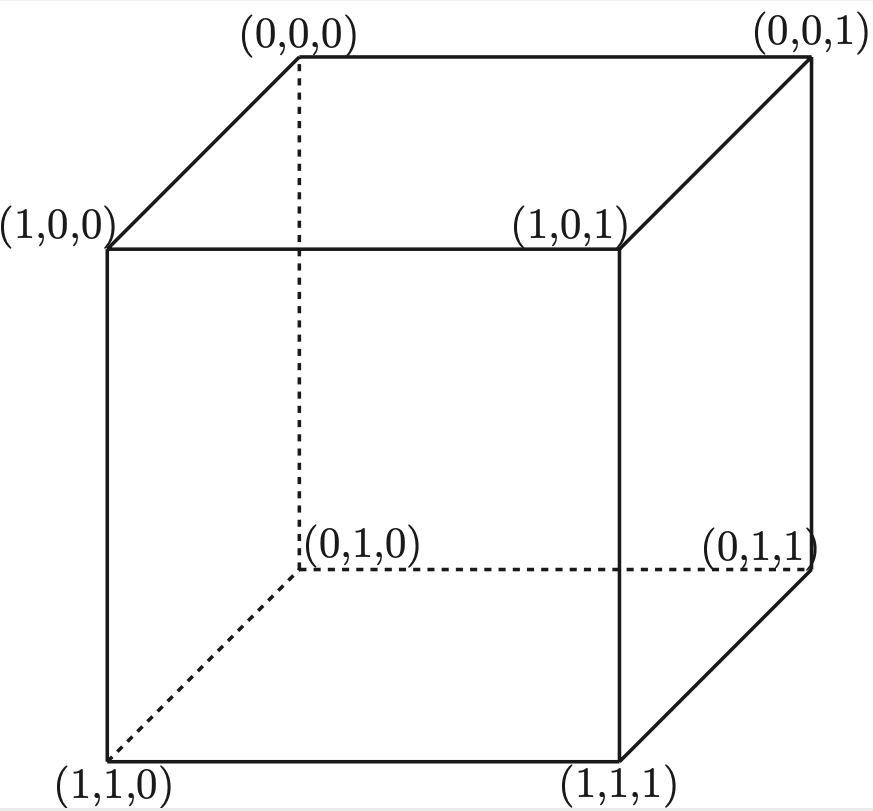
\includegraphics[scale=0.6]{images/visual-dist-hamming.png}
    \end{center}
    \caption{Hamming distance over $ (\FF_2)^3 $}
              \label{fig-visual-dist-hamming}
\end{figure}
 
We could have chosen another distance, but it turns out that the Hamming distance is both simple enough to allow efficient calculations, and precise enough to fully account for the efficiency of the codes.
% ------------------------------------------------- -----
% ------------------------------------------------- -----
% sub-section - Presentation of linear codes                           
% ------------------------------------------------- -----
% ------------------------------------------------- -----
\subsection{Presentation of linear codes}
\label{sect2-presentation-cyclic-codes}
 
 
\index{Code!linear} \index{Code!cyclic} \index{Ideal!of a code} After the choice of the alphabet (which is therefore a finite field $ \FF_q $), the second hypothesis that we will do concerns the set of words that can be encoded. Indeed, it is obvious that the encoding operation will add information to the original message, therefore the set of \guill{valid} words (i.e. the words that we will be able to produce by encoding) will not occupy the entire space $ (\FF_q)^n $. Intuitively, we can see that the more space there is between valid words (i.e. code words), the more we will be able to distinguish them from each other, and therefore the more will be easy to spot any errors.
 
 
\index{Kissing Number} The search for a set $ \Cc \subset (\FF_q)^n $ presenting, for a given size $ | \Cc | $, the best weight distribution (in a sense to be specified, but intuitively, such that the words are as far apart as possible) is an extremely difficult problem. Thus, this research is closely linked to that of the most compact possible stacking of spheres, and to the famous \textit{Kissing Number} problem. For more details, refer to the article by \nompropre{Elkies} \cite{elkies-ams-1}. It is possible to define a set of constants characterizing with more or less finesse the distribution of the words of a code.
 
\begin{defn}[Distribution functions]
\index{Distribution!of weight} \index{Distribution!of distance} \label{notation-68} We denote by $ \{A_i\}_{i = 0}^n $ the \textit{distribution of weights} of a code $ \Cc \subset (\FF_q)^n $:
\begin{equation}
\label{eq-defn-weight-distribution}
\forall i = 0, \ldots, \, n, \quad A_i \eqdef \# \enscond{x \in \Cc}{w (x) = i}.
\end{equation}
We denote by $ \{B_i\}_{i = 0}^n $ the \textit{distance distribution} of $ \Cc $:
\begin{equation}
\label{eq-defn-repartition-distance}
\forall i = 0, \ldots, \, n, \quad B_i \eqdef \frac{1}{| \Cc |} \# \enscond{(x, \, y) \in \Cc}{d (x , \, y) = i}.
\end{equation}
It should be noted that the couples $ (x, \, y) $ are considered ordered, that is to say $ (x, \, y) \neq (y, \, x) $.
\end{defn}
 
 
\begin{rem}
We see that we have $ B_0 = 1 $, and that
\begin{equation*}
A_0 + \cdots + A_n = B_0 + \cdots + B_n = | \Cc |.
\end{equation*}
Moreover, if $ u $ is any vector of $ (\FF_q)^n $, the codes $ \Cc $ and $ \Cc + u $ have the same weight distribution. This is why in practice we assume that $ 0 \in \Cc $, even if $ \Cc $ is not linear.
\end{rem}
We will come back to the calculation and the study of these distributions in the Section~\ref{sect1-codes-correctors-duality}. To quantify this distribution in a simpler way, we introduce a very useful notion, that of \textit{minimal distance}.
 
\begin{defn}[Minimum distance]
\index{Minimum!distance} We denote by $ d $ the \textit{minimum distance} of the code $ \Cc $ considered, which is defined as follows:
\begin{equation*}
d \eqdef \min \enscond{d (x, \, y)}{x \neq y \in \Cc}.
\end{equation*}
\end{defn}
Intuitively, we realize that the greater this minimum distance, the more efficient the code will be, since the words will be more distant from each other. This choice is very partial, and in a way very pessimistic, since it only takes into account the smallest distance. However, it gives us conditions under which we are sure to correct an error, which is specified by the following definition.
 
\begin{defn}[Correction capability]
\index{Correction capacity} The \textit{correction capacity} $ t $ of a code $ \Cc $ is the maximum number of errors that it can correct. More precisely, if the sender sends a code word $ x \in \Cc $ through a network, and the receiver receives a word $ x'$ (which may be different from the word sent), then it must be able to find the original word if $ d (x, \, x') \leq t $.
\end{defn}
This means that the balls of radius $ t $ (for the Hamming distance) whose center is a code word must be disjoint from each other, or, in other words, that the words must be at a distance d'at least $ 2 t + $ 1 from each other. We therefore obtain the following result.
 
\begin{prop}
A $ \Cc $ code is $ t $ -corrector (i.e. it has a correction capacity of at least $ t $) if the minimum distance between two distinct words is greater than or equal to $ 2 t + $ 1. The correction capacity of the code is $ t = \lfloor (d-1) / 2 \rfloor $, where we have noted $ \lfloor x \rfloor $ the integer part of a real $ x $.
\end{prop}
 
 
 
To greatly simplify the search for efficient codes (for example with a large minimum distance $ d $), we are going to impose a very restrictive structure on the words of the code.
 
\begin{defn}[Linear code]
\index{Matrix!generator} \index{Code!linear} A linear code $ \Cc $ of size $ n $ and dimension $ m $ on $ \FF_q $ is a vector subspace of dimension $ m $ of $ (\FF_q)^n $. If we consider a matrix $ G $ (called \textit{generator matrix}) whose columns form a basis of $ \Cc $, we have
\begin{equation*}
\Cc = \enscond{G x}{x \in (\FF_q)^m}.
\end{equation*}
\end{defn}
\index{Code!non-linear} Note that there is no uniqueness in the choice of $ G $. Certainly, even an optimal linear code will at best be as good as the best nonlinear code (i.e. any code), and in practice it will be much worse. However, restricting ourselves to vector subspaces will make our research much more fruitful, and will also bring its share of efficient decoding algorithms. For example, the linearity property of $ \Cc $ allows us to calculate the minimum distance $ d $ much more simply:
\begin{equation*}
d \eqdef \min \enscond{d (x, \, y)}{x \neq y \in \Cc} = \min \enscond{w (x)}{x \neq 0 \in \Cc}.
\end{equation*}
In the same way, in the linear case, one notes that the distributions of weight and distance coincide. Unless explicitly stated otherwise, it is now assumed that the code $ \Cc $ is a linear code, of size $ n $ and dimension $ m $.
 
 
The first phase of the encoding operation consists in transforming the original message containing certain information into a word of the code $ \Cc $. This operation must be bijective. In the case of a linear code, it is very easy to achieve this. The simplest way to operate is to simply consider that our messages are \guill{small} vectors of $ (\FF_q)^m $, and that we send them on \guill{large} vectors of $ (\FF_q)^n $, simply by multiplying them on the left by the matrix $ G $. The matrix $ G $ is not chosen in a canonical way, but the choice of another base leads to a code having approximately the same properties (one speaks about isomorphic code).
 
\begin{rem}{(\upshape \textbf{Control matrix}).}
\label{rmk-matrices-control}
\index{Matrix!of control} A code of size $ n $ and dimension $ m $ on $ \FF_q $ can be seen as the kernel of a matrix $ H $ of size $ (nm) \times n $. We call this matrix a \textit{control matrix} of the code $ \Cc $; it allows to check if a vector $ x \in (\FF_q)^n $ belongs to the code since $ x \in \Cc \Leftrightarrow H x = 0 $. There is no uniqueness in the choice of $ G $.
\end{rem}
 
 
\begin{exmp}[Repetition code]
Take the simple example of the repeat code. It consists of repeating, for example, $ 4 $ times a symbol $ x \in \FF_2 $. The only two words in the code are $ (0000) $ and $ (1111) $. Generator $ G $ and control $ H $ matrices are for example
\begin{equation*}
G = \begin{pmatrix} 1 \\1 \\1 \\1 \end{pmatrix} \quad \quad \quad H = \begin{pmatrix} 1 & 1 & 0 & 0 \\1 & 0 & 1 & 0 \\1 & 0 & 0 & 1 \end{pmatrix}.
\end{equation*}
The dual code (concept specified a little later, definition \ref{defn-code-dual}) is made up of the vectors $ x \in (\FF_2)^4 $ such as $ \dotp{x}{[1111]} = $ 0. So it's simply the code of adding a parity bit to $ x \in \FF_2^3 $. It is noted that it suffices, except for a transposition, to exchange the generator and control matrices. On this subject, we can see the exercise \oldref{exo-matrices-generator-control}.
\end{exmp}
 
 
\begin{exmp}[Hamming code of length 7]
\label{exmp-code-hamming-7}
\index{Code!of Hamming} We consider the code of size $ 7 $ and dimension $ 4 $ on $ \FF_2 $ whose generator matrix is
\begin{equation*}
G \eqdef \begin{pmatrix} 1 & 1 & 0 & 1 & 0 & 0 & 0 \\0 & 1 & 1 & 0 & 1 & 0 & 0 \\0 & 0 & 1 & 1 & 0 & 1 & 0 \\0 & 0 & 0 & 1 & 1 & 0 & 1 \end{pmatrix}.
\end{equation*}
We can explain the 16 elements that make up the code:
\begin{equation*}
\begin{array}{c | c | c} \transp{x} & \transp{(G x)} & w (G x) \\[1mm] \hline{(0000)} &{(0000000)} & 0 \\[1mm]{(0100 )} & (0110100) & 3 \\[1mm]{(0001)} & (0001101) & 3 \\[1mm]{(1010)} & (1110010) & 4 \\[1mm]{(0110)} & (0101110) & 4 \\[1mm]{(0011)} & (0010111) & 4 \\[1mm]{(1101)} & (1010001) & 3 \\[1mm]{(0111)} & ( 0100011) & 3 \end{array} \quad \quad \begin{array}{c | c | c} \transp{x} & \transp{(G x)} & w (G x) \\[1mm] \hline (1000) & (1101000) & 3 \\[1mm] (0010) & (0011010) & 3 \\[1mm] (1100) & (1011100) & 4 \\[1mm] (1001) & (1100101) & 4 \\[1mm] (0101) & (0111001) & 4 \\[1mm] ( 1110) & (1000110) & 3 \\[1mm] (1011) & (1111111) & 7 \\[1mm] (1111) & (1001011) & 4 \end{array}
\end{equation*}
\index{Word weight} As we can see, each non-zero word of the code has a weight greater than 3, so the correction capacity of this code is 1. In addition, it has an interesting property: the 4 row vectors of the matrix $ G $ are deduced from each other by circular permutation. Consequently, the whole code is invariant by circular permutation. In the following, we will be interested in the algebraic properties of such codes, and we will see that we have very practical tools to build them, and, in certain cases, to decode them. The exercise \oldref{exo-codes-hamming} proposes to generalize the construction which has just been done, to give birth to a widely used family of codes, the \textit{Hamming codes}.
\end{exmp}
To end this paragraph, here is an important relationship between the various parameters of a code, which clearly shows the choice to be made between correction capacity and redundancy of the information transmitted.
 
\begin{prop}[Singleton bound]
\label{prop-borne-singleton}
\index{Singleton bound} Let $ \Cc $ be a linear correction code of length $ n $, of dimension $ m $, and of minimum distance $ d $. We then have
\begin{equation}
\label{eq-borne-singleton}
d \leq n + 1-m.
\end{equation}
\end{prop}
\begin{proof}
Let $ E $ be the subspace of $ (\FF_q)^n $ formed by vectors whose last $ m-1 $ components are zero. It is a space of dimension $ n-m + 1$.
 
We have $ \dim (\Cc) + \dim (E) = n + 1 $ which implies that $ \Cc \cap E \neq \{0\} $. So there exists a non-zero $ x $ element in $ \Cc $ whose last $ m-1 $ components are zero, therefore which satisfies $ w (x) \leq n + 1-m $. We therefore have the desired relationship from the definition of the minimum distance.
\end{proof}
 
 
\begin{rem}
\index{Code!MDS} \index{MDS} Codes which verify $ d = n + 1-m $ are called \textit{MDS codes} (for \textbf{M} aximum \textbf{D} istance \textbf{S} eparable, in English in the text), they are therefore optimal for the Singleton bound. The exercise \oldref{exo-polynomials-mds} studies these codes in detail.
\end{rem}
 
% ------------------------------------------------- -----
% ------------------------------------------------- -----
% sub-section - Cyclic codes                           
% ------------------------------------------------- -----
% ------------------------------------------------- -----
\subsection{Cyclic codes}
\label{sect2-cyclic-codes}
 
 
The problem with linear codes is that, in the general case, rapid decoding algorithms are not available, or else the latter require the storage of decoding tables which quickly become enormous for codes of respectable size. To remedy this problem, we will impose an additional structure on the linear codes.
 
\begin{defn}[Cyclic code]
\index{Code!cyclic} A code $ \Cc $ of size $ n $ on $ \FF_p $ is said to be cyclic if it is stable by circular shift, that is to say
\begin{equation*}
\forall a = \transp{(a_0, \ldots, \, a_{n-1})} \in \Cc, \quad \wt{a} \eqdef \transp{(a_{n-1}, a_0, \ldots, \, a_{n-2})} \in \Cc.
\end{equation*}
\end{defn}
A very convenient way to represent the words of a cyclic code is to consider them as elements of the $ \FF_p $ -algebra $ \Aa $ of dimension $ n $ that is $ \FF_p [X] / (X^n-1) $. We therefore consider that a word $ a $ is in fact a polynomial of degree at most $ n-1 $ (we choose a modulo representative $ X^n-1 $), denoted $ a_0 + a_1 X + \cdots + a_{n-1} X^{n-1} $. We then notice that
\begin{equation*}
\wt{a} = a_{n-1} + a_0 X + \cdots + a_{n-2} X^{n-1} = X a + a_{n-1} (X^n - 1).
\end{equation*}
\index{Ideal} So modulo $ X^n-1 $ (that is, in $ \Aa $), we have $ \wt{a} = X a $. The code $ \Cc $ is stable by multiplying by $ X $. As it is also a vector space, by linearity, we deduce that it is in fact stable by multiplication by any polynomial $ P \in \Aa $. This means that it is an ideal of the ring $ \Aa $. We know that the ideals of $ \Aa $ are in bijection with the ideals of $ \FF_p [X] $ which contain the ideal generated by $ X^n-1 $. Since the ring of polynomials $ \FF_p [X] $ is principal, an ideal of $ \FF_p [X] / (X^n-1) $ is generated by a unique unit polynomial which must additionally be a divisor of $ X^n-1 $.
 
 
\index{Polynomial!generator} If we denote by $ P $ the generator polynomial of the code $ \Cc $, we have, denoting $ s \eqdef \deg (P) $,
\begin{equation*}
\Cc = \enscond{PQ \; \mod{X^n-1}}{Q \in \FF_p [X]} = \enscond{PQ}{\deg (Q) \leq ns-1}.
\end{equation*}
The code $ \Cc $ is therefore of length $ n $ and of dimension $ ns $. The encoding operation is even simpler than for a linear code. The information that we want to transmit, instead of being contained in a vector of size $ ns $, is this time represented by a polynomial of degree at most $ ns-1 $ (but it's the same thing) . To obtain a word of the code that we are going to send over a network, it suffices to multiply this polynomial by the generator polynomial $ P $.
 
 
\index{Convolution!circular} \index{Matrix!circulating} We can now make a connection with the ideas that we introduced during the study of the Fourier transform on a cyclic group, and more particularly during the research rapid polynomial multiplication techniques (Section~\ref{sect1-calculations-products}). We have already noticed that the multiplication by a polynomial modulo $ X^n-1 $ corresponds to the computation of a cyclic convolution of vectors of size $ n $ (the equation \eqref{eq-prod-cyclic-polynomial}, shows very clearly the reconciliation). We can write the encoding operation of a vector $ x \in (\FF_p)^{ns} $ as the circular convolution $ x * y $ where we denote $ y $ the vector of the coefficients of the polynomial $ P $ . You should add zeros at the end of each of the vectors so that they reach the size $ n $. The generator matrix $ G $ of the code therefore corresponds to a circulating matrix as we explain in the exercise \oldref{exo-circulating-matrix}.
 
 
In Section~\ref{sect1-calculations-products}, we were only interested in calculations for polynomials of $ \CC [X] $. But this limitation was only justified because we did not have a Fourier transform on a field other than $ \CC $. Thanks to the construction of the \ref{sect2-trans-cyclotomic-field} paragraph, this limitation is lifted, and we are able to perform a Fourier transform with values in the field $ \FF_p $ (even if the latter, let us recall- le, requires to pass in a larger field, which one noted $ \FF_{p^r} $). So by taking the formula for calculating the cyclic convolution product \eqref{eq-prod-cyclic-polynomial}, we see that we can quickly perform the coding operation, of course using an FFT algorithm to perform the Fourier transform.

% ------------------------------------------------- -----
% ------------------------------------------------- -----
% sub-section - Construction of BCH codes                           
% ------------------------------------------------- -----
% ------------------------------------------------- -----
\subsection{Construction of BCH codes}
\label{sect2-codes-BCH}
 
 
\index{Code!BCH} \index{Distance!assigned} In this paragraph, we will present a class of cyclic codes named \textit{BCH codes}, from the name of their inventors, \nompropre{Bose}, \nompropre{Chaudhuri } and \nompropre{Hocquenghem}. The construction makes full use of the decomposition of cyclotomic polynomials explained in Paragraph~\ref{sect2-cyclotomic-field}. The major advantage of these codes, besides their simple description using the Fourier transform, is that we explicitly have a lower bound of their correction capacity. This allows the code parameters to be adjusted as needed. Moreover, we will see in Paragraph~\ref{sect2-decodage-bch} that we have an efficient decoding algorithm, which makes these codes usable in a practical way.
 
 
We are going to build a generator polynomial of a cyclic code using the cyclotomic fields presented in Paragraph~\ref{sect2-cyclotomic-field}. Indeed, since we are interested in the divisors of the polynomial $ X^n-1 $, it is natural to consider the modulo $ p $ behavior of the cyclotomic polynomials $ \Phi_n $. In the following, we suppose that $ \PGCD (n, \, p) = 1 $ (see the remark \ref{rmk-cyclotomy-cas-special} in the opposite case). Recall that if we denote by $ r $ the order of $ p $ in the multiplicative group $ (\ZZ/n \ZZ)^* $, then $ K \eqdef \FF_{p^r} $ is a breaking field of the polynomial $ \Phi_n $. This therefore allows us to choose $ \alpha \in K $ an \ordin{n}{ième} primitive root of unity (such a choice, let us recall, results from the choice of an irreducible factor of $ \Phi_n $ modulo $ p $, which is of degree $ r $). We will then choose the generator polynomial $ P $ in the form
\begin{equation}
\label{eq-defn-pol-gen-codes-bch}
P = \prod_{i \in I}{(X- \alpha^i)},
\end{equation}
where $ I $ is a subset of $ \{1, \ldots, \, n-1\} $ to be determined. Indeed, in order to obtain a cyclic code on $ \FF_p $, the polynomial $ P $ must still have coefficients in $ \FF_p $, and not simply in $ K $. Here is a simple but important lemma which gives us a way to see if a polynomial belongs to $ \FF_p [X] $.
 
\begin{lem}
A polynomial $ Q \in K [X] $ belongs to $ \FF_p [X] $ if and only if it satisfies $ Q (X^p) = Q (X)^p $.
\end{lem}
\begin{proof}
\index{Morphism!of Frobenius} We know that an element $ y \in K $ belongs to the prime sub-field $ \FF_p $ if and only if it satisfies $ y^p = y $ (use the arguments of the proof of the proposition \ref{prop-cyclotomy-fp} considering the roots of $ X^pX $). Using the \textit{Frobenius morphism} $ x \mapsto x^p $ from $ K $ in $ K $, we see that if we denote by $ Q = a_0 + \cdots + a_k X^k $, we have
\begin{equation}
\label{eq-condition-membership-fp}
Q (X)^p = (a_0 + a_1 X + \cdots + a_k X^k)^p = a_0^p + a_1^p X^p + \cdots + a_k^p (X^{p})^k .
\end{equation}
Thus, to say that $ a_i^p = a_i $ for $ i = 0, \ldots, \, k $ therefore amounts to saying that $ Q (X)^p = Q (X^p) $.
\end{proof}
The following proposition then gives us a criterion which will allow us to effectively choose the set $ I $.
 
\begin{prop}
\label{prop-cns-cyclotomic-class}
The polynomial $ P $ belongs to $ \FF_p [X] $ if and only if $ I $ is stable by multiplication by $ p $ modulo $ n $.
\end{prop}

\begin{proof}
If $ P \in \FF_p [X] $ and if $ \beta $ is a root of $ P $, we see with the previous lemma that $ P (\beta^p) = P (\beta)^p = 0 $, consequently the set $ I $ is stable by multiplication by $ p $. \\Conversely, if $ I $ is stable by multiplication by $ p $, then
\begin{equation*}
P (X)^p = \prod_{i \in I}{(X- \alpha^i)^p} = \prod_{i \in I}{(X^p- \alpha^{ip})} = \prod_{i \in I}{(X^p- \alpha^{i})} = P (X^p),
\end{equation*}
so we have $ P \in \FF_p [X] $.
\end{proof}
We finally have in hand all the tools necessary to define the BCH codes.
 
\begin{defn}[BCH codes]
\index{Distance!assigned} We call \textit{code BCH} of assigned distance $ \delta $ a cyclic code whose generator polynomial is obtained by the equation \eqref{eq-defn-pol-gen-codes-bch} , where $ I $ denotes the smallest cyclotomic class (i.e. the smallest set stable by multiplication by $ p $ modulo $ n $) containing the set of indices $ \{1, \ldots, \, \delta-1\} $.
\end{defn}

Before going further in the investigation of the properties of these codes, we will give a simple way to calculate the generator polynomial once we know the decomposition on $ \FF_p $ of the cyclotomic polynomial $ \Phi_n $. To do this, we will consider the simplest cyclotomic classes that are, i.e. the classes generated by a single element $ k \in \{0, \ldots, \, n-1\} $:
\begin{equation}
\label{eq-defn-pol-cyclotomic-classes}
I_k \eqdef \{k, \, kp, \ldots, \, kp^{s-1}\},
\end{equation}
where we denote by $ s $ the smallest integer such as $ kp^s = k $ (in the case where $ k = 1 $, we have of course $ s = r $ degree of $ P $). More elegantly, we can consider the equivalence relation $ \sim $ on $ \ZZ/n \ZZ $:
\begin{equation*}
\forall (x, \, y) \in (\ZZ/n \ZZ)^2, \quad (x \sim y) \Leftrightarrow \left(\exists i, \; x = yq^i \right).
\end{equation*}
The cyclotomic classes are then the equivalence classes of $ \ZZ/n \ZZ $ for this relation, and form a partition of $ \{0, \ldots, \, n-1\} $. We notice that the polynomial
\begin{equation}
\label{defn-pol-classes-cyclo-codes-bch}
P_k \eqdef \prod_{i \in I_k}{(X- \alpha^i)}
\end{equation}
is, according to the proposition \ref{prop-cns-cyclotomic-class}, an irreducible polynomial of $ \FF_p [X] $ of degree $ s $ admitting $ \alpha^k $ as root. Consequently, it is the minimal polynomial of $ \alpha^k $. The following description of the generator polynomial of the code is then easily obtained.
 
\begin{prop}
The polynomial $ P $ generator of an assigned distance BCH code $ \delta $ is the PPCM of the polynomials $ P_1, \ldots, \, P_{\delta-1} $ defined by the equation \eqref{defn-pol-classes-cyclo-codes-bch}.
\end{prop}
 
 
\begin{exmp}
Here is an example of the use of cyclotomic classes, in the case of codes on the field $ \FF_2 $. We want to build codes of length $ n \eqdef 2^5-1 = $ 31, so we have here $ r = 5 $. Here is the list of irreducible factors of $ X^n - 1 $ on $ \FF_2 $:
\begin{equation*}
\begin{array}{l | l} \text{Polynomial:} & \text{Cyclotomic class:} \\[1mm] \hline \\[- 3mm] P_0 \eqdef X + 1 & I_0 \eqdef \{0\} \\P_1 \eqdef 1 + X + X^2 + X^4 + X^5 & I_1 \eqdef \{1, \, 2, \, 4, \, 8, \, 16\} \\P_3 \eqdef 1 + X^3 + X^5 & I_3 \eqdef \{3, \, 6, \, 12, \, 24, \, 17\} \\P_5 \eqdef 1 + X + X^2 + X^3 + X^5 & I_5 \eqdef \{5, \, 10, \, 20, \, 9, \, 18\} \\P_{11} \eqdef 1 + X + X^2 + X^3 + X^4 + X^5 & I_{11} \eqdef \{11, \, 22, \, 13, \, 26, \, 21\} \\P_{14} \eqdef 1 + X^2 + X^5 & I_{14} \eqdef \{14, \, 28, \, 25, \, 19, \, 7\} \\P_{15} \eqdef 1 + X + X^3 + X^4 + X^5 & I_{15 } \eqdef \{15, \, 30, \, 29, \, 27, \, 23\} \end{array}
\end{equation*}
In accordance with what we advised to do to build a cyclotomic field, we arbitrarily choose an irreducible factor of higher degree, for example $ P_1 $, and we denote $ \alpha $ one of its roots, which will therefore be a primitive root of unity, and which can be seen as an element of $ K \eqdef \FF_{2^5} $. The polynomial $ P_0 $ is thus the minimal polynomial of $ 1 $ associated with the class $ I_0 $, the polynomial $ P_3 $ the minimal polynomial of $ \alpha^3 $ associated with the class $ I_3 $, etc. To build a BCH code, it suffices to judiciously choose certain cyclotomic classes, and to multiply the corresponding polynomials between them, to obtain the generator polynomial of the code. For example, if we choose the classes $ I_1 $ and $ I_3 $, we obtain the cyclotomic class $ \{1, \, 2, \, 3, \, 4, \, 6, \, 8, \, 12, \, 16, \, 17, \, 24\} $, and we see that it is the smallest class containing $ \{1, \, 2, \, 3, \, 4\} $. Therefore, the polynomial
\begin{equation*}
P_1 (X) P_2 (X) = 1 + X + X^2 + X^3 + X^5 + X^6 + X^8 + X^9 + X^{10}
\end{equation*}
\index{Maple@\Maple{}} generates an assigned distance BCH code $ 5 $. More substantial examples are easily constructed from the \Maple{} program presented in Section~\ref{sect1-listing-decoding-bch}, and which allows you to construct BCH codes of arbitrary parameters. Before studying the relationships that can exist between $ \delta $ and the correctness of the code, we will introduce a matrix formalism which will naturally lead to the use of the Fourier transform.
\end{exmp}
 
 
 
The polynomial $ P $ that we have just built is the polynomial of $ \FF_p [X] $ of lowest degree having for root $ \alpha, \, \alpha^2, \ldots, \, \alpha^{\delta -1} $. Consequently, the polynomials $ Q \in \FF_p [X] $ which constitute the code are therefore the polynomials of degree less than $ n $ which satisfy
\begin{equation}
\label{eq-condition-defn-codes-bch}
\forall i \in \{1, \ldots, \, \delta-1\}, \quad Q (\alpha^i) = 0.
\end{equation}
Matrix, if we denote by $ q = \{q_0, \ldots, \, q_{n-1}\} $ the vector made up of the coefficients of $ Q $, the previous equation is equivalent to
\begin{equation*}
A q = 0 \quad \quad \text{with} \quad \quad A \eqdef \left\{\alpha^{ij} \right\}_{i = 0, \ldots, \, \delta-1}^{j = 0, \ldots, \, n-1} \in M_{\delta-1, n-1} (K).
\end{equation*}
We can also use the language of the discrete Fourier transform. We denote by $ \Ff $ the transform obtained with the root \ordin{n}{ième} primitive $ \alpha^{-1} $, as defined in the equation \eqref{eq-defn-tfd-finite-field} (taking $ \zeta = \alpha^{-1} $). The condition \eqref{eq-condition-defn-codes-bch} then becomes
\begin{equation*}
\forall i \in \{1, \ldots, \, \delta-1\}, \quad Q (\alpha^i) = \wh{q}[i] \eqdef \Ff(q) [i] = 0.
\end{equation*}
In other words, the code is now defined in terms of spectral conditions, more precisely, by the nullity of $ \delta-1 $ components of the transformed vector. By using the notion of control matrix introduced in the remark \ref{rmk-matrices-control}, we can therefore say that the $ \delta-1 $ lines of the Fourier matrix constitute a control matrix for the BCH code considered .
 
\begin{rem}{(\upshape \textbf{Duality and minimum distance}).}
\index{Support} Intuitively, we begin to understand what effect the use of a high $ \delta $ can have. By forcing the transformed vector to have a very reduced support (by the nullity conditions that we have just explained), we also force the original vector (that is to say a word of the code) to have a lot of non-zero components. This is in agreement with the principle of discrete uncertainty, such as it is stated in the exercise \oldref{exo-principle-uncertainty-discrete} (the result extends without difficulty to the case of the Fourier transform with value in a finite field). As a result, we will obtain a large minimum distance for the code, which will therefore have a high correction rate. Once again, we see the principle of duality that we mentioned in Paragraph~\ref{sect2-duality-time-frequency} appear. Let us clarify all this by giving a result which gives us a lower bound on the code correction rate.
\end{rem}
 
 
\begin{prop}[Minimum distance of a BCH code]
\label{prop-dist-minimal-code-bch}
The minimum distance of the constructed $ \Cc $ code is at least $ \delta $.
\end{prop}
\begin{proof}
\index{Matrix!of Vandermonde} It is a matter of showing that the ball with center $ 0 $ and radius $ r \eqdef \delta-1 $ contains only $ 0 $. Let $ Q \in \Cc $, which is therefore a polynomial of degree at most $ n-1 $. We assume that it is in this ball, so it has at most $ r $ non-zero coefficients. If we write it in the form
\begin{equation*}
Q (X) = a_1 X^{b_1} + \cdots + a_{r} X^{b_{r}},
\end{equation*}
the fact that it belongs to $ \Cc $ implies
\begin{equation*}
\forall i \in \{1, \ldots, \, r\}, \quad Q (\alpha^i) = a_1 \alpha^{i b_1} + \cdots + a_{r} \alpha^{i b_{r}}.
\end{equation*}
This means that the vector $ a \eqdef \{a_1, \ldots, \, a_r\} \in \CC^r $ satisfies the linear system $ M a = 0 $, where $ M \eqdef \left\{\alpha^{i b_j} \right\}_{1 \leq i, j \leq r} $. We see that it is a matrix of \textit{Vandermonde}, and as the $ \alpha^{b_j} $ are distinct, it is invertible. This therefore implies that $ a = 0 $, which had to be demonstrated.
\end{proof}
In the following, to simplify the explanations, we will assume that $ \delta = 2 t + 1 $, so that the code is at least $ t $ -corrector, since then $ \lfloor (\delta-1) / 2 \rfloor = t $. We can notice that in the case where $ p = 2 $, we can always assume that $ \delta = 2 t + 1 $, since the part $ \{1, \ldots, \, \delta-1\} $ can be assumed to be stable by multiplying by $ p = $ 2.
% ------------------------------------------------- -----
% ------------------------------------------------- -----
% sub-section - Fourier transform decoding                           
% ------------------------------------------------- -----
% ------------------------------------------------- -----
\subsection{Fourier transform decoding}
\label{sect2-decodage-bch}
 
 
\index{Decoding} \index{Extended Euclidean!algorithm} One of the advantages of the BCH codes that we have just constructed is that we have simple and fast algorithms to decode them. For example a method using \textit{the extended Euclidean algorithm} is presented in the book of \nompropre{Demazure} \cite{demazure}. In this paragraph, we will present another algorithm, based on the description of the code in terms of a discrete Fourier transform.
 
 
Assume that we have just received a code word $ x'= x + \epsilon $, where $ x $ represents the original word, and $ \epsilon $ the transmission error. Our goal is to find the word $ x $, or equivalently, to determine the error $ \epsilon $, which we write in the form
\begin{equation*}
\epsilon (X) \eqdef \epsilon_0 + \epsilon_1 X + \cdots + \epsilon_{n-1} X^{n-1}.
\end{equation*}
$ \epsilon $ is unknown, but in order to have a chance to solve this problem, we still assume that it checks $ w (\epsilon) \leq t $. We recall that we have assumed that $ \delta = 2t + 1 $, so that the proposition \ref{prop-dist-minimal-code-bch} assures us that the problem is well posed. But we need to find a way to solve it effectively.
 
 
We know, by the definition of the code in terms of Fourier transform, that
\begin{equation*}
\forall i \in \{1, \ldots, \, 2 t\}, \quad \wh{\epsilon}[i] = \wh{x'} | i] - \wh{x} | i] = \wh{x'} | i].
\end{equation*}
We therefore know how to calculate $ 2t = \delta - 1 $ coefficients of the vector $ \wh{\epsilon} $. The others still have to be calculated, in order to be able, by inverse Fourier transform, to find the error $ \epsilon $. To do this, we introduce an intermediate unknown, another polynomial.
 
\begin{defn}[Error locator polynomial]
\index{Polynomial!error locator} We denote
\begin{equation*}
J \eqdef \enscond{i \in \{0, \ldots, \, n-1\}}{\epsilon_i \neq 0}.
\end{equation*}
We have already assumed that $ \Card (J) \leq t $, since $ w (x) \leq t $. We call \textit{error locator polynomial}, and we denote by $ \sigma $, the polynomial
\begin{equation*}
\sigma (Z) \eqdef \prod_{i \in J}{\left(1 - \alpha^i Z \right)} \eqdef 1 + \sigma_1 Z + \cdots + \sigma_{t} Z^t.
\end{equation*}
\end{defn}
The error locator polynomial is therefore a polynomial of degree at most $ t $, comprising $ t $ a priori unknown coefficients. The inverses of the roots of $ \sigma $ correspond to $ \alpha^i $, where $ i $ is the position of an error in the transmitted word.
 
 
We notice that the polynomials $ \epsilon $ and $ \wh{\sigma} $ have an orthogonality property, in the sense that \begin{rs}
\item if $ s \in J $, $ \wh{\sigma}[s] \eqdef \sigma (\alpha^{- s}) = 0 $ and $ \epsilon [s] \neq 0 $.
\item if $ s \notin J $, $ \wh{\sigma}[s] \eqdef \sigma (\alpha^{- s}) \neq 0 $ and $ \epsilon [s] = 0 $.
\end{rs} We can summarize this by the equation $ \wh{\sigma} \cdot \epsilon = 0 $, where we denote by $ \cdot $ the multiplication coefficient by coefficient of the polynomials. Using the convolution theorem (which is still valid for a transform over a finite field, as explained by the proposition \ref{prop-prtes-tfd-finite-field}), we obtain by passing to the Fourier transform l'convolution equation
\begin{equation*}
\Ff^{-1} (\wh{\sigma} \cdot \epsilon) = \sigma * \Ff^{-1} (\epsilon) = \frac{1}{N} \sigma * \wh{\epsilon}^{\sharp} = 0.
\end{equation*}
We recall that $ \wh{\epsilon}^{\sharp} $, considered as a vector, is obtained according to the definition \ref{defn-symmetry-operator}. So this is the vector $ \{\wh{\epsilon}[0], \, \wh{\epsilon}[n-1], \ldots, \, \wh{\epsilon}[1]\} $ . Then it suffices to replace the convolution of vectors by the modulo $ Z^{n} -1 $ multiplication of the polynomials, to obtain a fairly complex polynomial equation:
\begin{equation*}
\left(1 + \sigma_1 Z + \cdots + \sigma_t Z^t \right) \left(\wh{\epsilon}_0 + \wh{\epsilon}_{n-1} Z + \cdots + \wh{\epsilon}_1 Z^{n-1} \right) \; \mod{Z^n - 1} = 0.
\end{equation*}
We can replace this polynomial equation in two systems of linear equations:
\begin{equation*}
(\Ss_1) \left\{ \begin{array}{lllllllllll} \wh{\epsilon}_0 & + & \wh{\epsilon}_1\sigma_1 & + & \wh{\epsilon}_2\sigma_2 & + & \ldots & + & \wh{\epsilon}_t\sigma_t & = & 0 \\ \wh{\epsilon}_{n-1} & + & \wh{\epsilon}_0\sigma_1 & + & \wh{\epsilon}_1\sigma_2 & + & \ldots & + & \wh{\epsilon}_{t-1}\sigma_t & = & 0 \\ \ldots & & & & & & & & & & \\ \wh{\epsilon}_{n-i} & + & \wh{\epsilon}_{n-i+1}\sigma_1 & + & \wh{\epsilon}_{n-i+2}\sigma_2 & + & \ldots & + & \wh{\epsilon}_{t-i}\sigma_t & = & 0 \\ \ldots & & & & & & & & & & \\ \wh{\epsilon}_{t+1} & + & \wh{\epsilon}_{t+2}\sigma_1 & + & \wh{\epsilon}_{t+3}\sigma_2 & + & \ldots & + & \wh{\epsilon}_{2t+1}\sigma_t & = & 0 \end{array} \right.
\end{equation*}
 
\begin{equation*}
(\Ss_2) \left\{ \begin{array}{lllllllllll} \wh{\epsilon}_t & + & \wh{\epsilon}_{t+1}\sigma_1 & + & \wh{\epsilon}_{t+2}\sigma_2 & + & \ldots & + & \wh{\epsilon}_{2 t}\sigma_t & = & 0 \\ \ldots &&&&&&&&&& \\ \wh{\epsilon}_2 & + & \wh{\epsilon}_3\sigma_1 & + & \wh{\epsilon}_4\sigma_2 & + & \ldots & + & \wh{\epsilon}_{t+2}\sigma_t & = & 0 \\ \wh{\epsilon}_1 & + & \wh{\epsilon}_2\sigma_1 & + & \wh{\epsilon}_3\sigma_2 & + & \ldots & + & \wh{\epsilon}_{t+1}\sigma_t & = & 0 \end{array} \right.
\end{equation*}
As we know the values of $ \wh{\epsilon}_1, \ldots, \, \wh{\epsilon}_{2t} $, the system $ (\Ss_2) $ allows us to calculate $ \sigma_1, \ldots , \, \sigma_t $ in a very simple way (the system is actually triangular). We can now use the system $ (\Ss_1) $ to find $ \wh{\epsilon}_0, \, \wh{\epsilon}_{2t}, \ldots, \, \epsilon_{n-1} $, since we have $ nt $ equations for only $ n-2t $ unknowns.
 
\begin{rem}
Once we have calculated $ \sigma_1, \ldots, \, \sigma_t $ (by solving the system $ \Ss_2 $), we have another alternative. Indeed, since we know $ \sigma $, it is possible to test, for $ i = 0, \ldots, \, n-1 $, if $ \sigma (\alpha^{- i}) = 0 $, and thus to detect the positions of the errors. The system $ \Ss_1 $ being very easy to solve, the two methods are however equivalent.
\end{rem}
 
 
 
This decoding method is implemented using \Maple{} in Paragraph~\ref{sect1-listing-decoding-bch}. It uses the routines defined in Paragraph~\ref{sect1-listing-transform-finite-body}, to perform Fourier transforms with value in $ \FF_p $.
% ------------------------------------------------- -----
% ------------------------------------------------- -----
% ------------------------------------------------- -----
% section - Correction codes and duality on a finite abelian group                           
% ------------------------------------------------- -----
% ------------------------------------------------- -----
% ------------------------------------------------- -----
\section{Correction codes and duality on a finite abelian group}
% \addcontentsline{toc}{section}{Corrector and duality codes on a finite abelian group}
\label{sect1-codes-correctors-duality}
 
 
In this last part, we will see how the tools developed in the previous chapters can be useful to study the characteristics of a code. Thus, the notions of orthogonality, of duality on a finite group, and of course the various transformations which are linked to all these notions (Walsh and Fourier transform among others) will intervene in turn.
 
 
The fundamental book on the combinatorial study of corrective codes is that of \nompropre{MacWilliams} and \nompropre{Sloane} \cite{macwilliams-codes-correcteurs-1}. This paragraph takes up the main results on duality, by exposing them through the language which is now familiar to us, that of group algebras $ \CC [G] $ and characters. It is important to take a look at the proposed exercises, the exercise \oldref{exo-codes-hadamard} for example, proposes a construction of very efficient nonlinear codes.

% ------------------------------------------------- -----
% ------------------------------------------------- -----
% sub-section - Enumerator polynomials of weight                           
% ------------------------------------------------- -----
% ------------------------------------------------- -----
\subsection{Enumerator polynomials of weight}
\label{sect2-polynomials-enumerators-weight}
 
In the following, we will restrict ourselves to the study of binary codes, but all the results given extend to the case of codes defined on any finite field $ \FF_q $. The appropriate additive characters must be used, and we refer to the exercise \oldref{exo-generalization-mac-williams} to obtain the corresponding MacWilliams formula. In the following pages, we will consider $ \Cc $, a linear code on $ \FF_2 $, of size $ n $ and dimension $ m $.
 
\begin{defn}[Orthogonal of a code]
\label{defn-code-dual}
\index{Code!orthogonal} \index{Orthogonal!of a code} \label{notation-69} We recall that we have a canonical non-degenerate symmetric bilinear form on $ (\FF_2)^n $, already introduced in Paragraph~\ref{sect2-application-id-mac-williams}:
\begin{equation}
\label{eq-fbs-canonical-f2}
\forall (x, \, y) \in (\FF_2)^n \times (\FF_2)^n, \quad \dotp{x}{y} \eqdef \sum_{i = 0}^{n-1 }{x_i y_i}.
\end{equation}
We denote by $ \Cc^\bot $ the \textit{orthogonal code} of $ \Cc $ for this bilinear form, that is to say:
\begin{equation*}
\Cc^\bot \eqdef \enscond{x \in (\FF_2)^n}{\forall y \in \Cc, \; \dotp{x}{y} = 0}.
\end{equation*}
It is therefore a code of size $ n $ and dimension $ nm $.
\end{defn}
 
 
\begin{rem}{(\upshape \textbf{Dual code}).}
\index{Code!dual} \index{Dual!of a code} We also speak of \textit{dual code} to denote $ \Cc^\bot $. This name is very natural, since we have already seen in Section~\ref{sect1-fish-formula} the similarities (and even the identity in the case of $ (\FF_2)^n $) between the notions of orthogonality , duality over a vector space, and duality over a finite abelian group.
\end{rem}
 
 
\begin{rem}{(\upshape \textbf{Auto-dual codes}).}
\index{Code!auto-dual} \index{Auto-dual} \index{Code!auto-orthogonal} It is important to emphasize that, even if we still have $ \dim (\Cc) + \dim (\Cc^\bot) = n $, a code and its dual are usually not additional. It sometimes happens that we have $ \Cc \subset \Cc^\bot $, and we speak of code \textit{auto-orthogonal}. When we have $ \Cc^\bot = \Cc $, we say that the code is \textit{auto-dual}. This notion is studied in more detail in the exercise \oldref{exo-codes-autoduaux}. The fact that the generator matrix can at the same time serve as a control matrix makes it possible to simplify the decoding procedures.
\end{rem}
 
 
\begin{defn}[Enumerator polynomial]
\label{defn-polynomial-enumerator-code}
\index{Polynomial!enumerator} We denote by $ W_\Cc \in \ZZ [X, \, Y] $ the \textit{enumerator polynomial of weight} of $ \Cc $, which is defined by
\begin{equation*}
W_\Cc (X, \, Y) \eqdef \sum_{i = 0}^{n}{A_i X^{ni} Y^i},
\end{equation*}
where we noted $ \{A_i\}_{i = 0}^n $ the weight distribution of $ \Cc $, defined by the equation \eqref{eq-defn-weight-distribution}.
\end{defn}
The fundamental result for the determination of the enumerator polynomial is the identity of \textit{MacWilliams}, already demonstrated in the theorem \ref{thm-id-mac-williams}, and which we recall here.
 
\begin{thm}[MacWilliams identity]
\label{thm-id-mac-williams-correctors-codes}
\index{Identity!of MacWilliams} \index{MacWilliams@\nompropreindex{MacWilliams}} We have
\begin{equation*}
W_{\Cc^{\bot}} (X, \, Y) = \frac{1}{2^m} W_{\Cc} (X + Y, \, XY).
\end{equation*}
\end{thm}
Several exercises propose using all these tools in order to obtain information of a combinatorial nature on the corrective codes. The exercise \oldref{exo-pol-enumerateur-hamming} proposes to calculate the enumerator polynomials for the Hamming codes. The \oldref{exo-polynomials-mds} exercise studies the distribution of the weights of words in the \textit{MDS} codes (ie those which are optimal for the Singleton bound). Finally, the exercise \oldref{exo-codes-autoduaux} studies auto-dual codes, using invariant theory techniques to exploit MacWilliams identities.

% ------------------------------------------------- -----
% ------------------------------------------------- -----
% sub-section - Algebra of a group and corrective codes                           
% ------------------------------------------------- -----
% ------------------------------------------------- -----
\subsection{Algebra of a group and corrective codes}
\label{sect2-algebre-group-correctors-codes}
 
\index{Algebra!of a group} All these combinatorial techniques are therefore very useful for analyzing the structure of a linear code. However, they fall short when it comes to studying a nonlinear code, i.e. studying the distribution of the words of a set $ \Cc \subset (\FF_2)^n $ . We recall that the essential notion to study a nonlinear code is not the weight distribution $ \{A_i\}_{i = 0}^n $ but the distance distribution $ \{B_i\}_{i = 0}^n $, defined by the equation \eqref{eq-defn-repartition-distance}. In the nonlinear case, these two distributions do not coincide, and it can be very complex to determine them. However, we will see that by using the Fourier transform on the algebra $ \CC [(\FF_2)^n] $, we can obtain a lot of information about $ \Cc $. For convenience, we denote by $ G \eqdef(\FF_2)^n $, which can be seen as an additive group. We recall that $ \CC [G] $ denotes the algebra of functions from $ G $ in $ \CC $. The characters of $ G $ are denoted, for $ a \in G $,
\begin{equation*}
\chi_a: \func{G}{\CC^*}{x}{(-1)^{\dotp{a}{x}}}.
\end{equation*}
We recall the definition of the Fourier transform of $ f \in \CC [G] $, already given in \eqref{eq-transf-fourier-grpe-abelien}:
\begin{equation*}
\wh{f}: \func{G}{\CC}{a}{\sum_{x \in G}{\chi_a (x) f(x)}}.
\end{equation*}
With these definitions in mind, let's explain how we can represent a set of vectors of $ (\FF_2)^n = G $ as a function of $ \CC [G] $.
 
\begin{defn}[Indicator function]
\index{Function!indicator} Let $ \Cc \subset G $ (which is not necessarily a linear code). We define the indicator function of $ \Cc $ by
\begin{equation*}
f_{\Cc} \eqdef \sum_{x \in \Cc}{\delta_x}.
\end{equation*}
This is the function that is worth $ 1 $ over $ \Cc $, and zero everywhere else. We can thus identify the subsets of $ G $ (that is to say the arbitrary codes) with functions of $ \CC [G] $.
\end{defn}

These indicator functions are studied in detail in the exercise \oldref{exo-indicator-functions}. This exercise makes in particular the link between the spectral properties of the function $ f_{\Cc} $ and the \guill{regularity} of $ \Cc $. Let us dwell for a moment on the case of linear codes. The question that naturally arises is whether there is a relationship between the indicator function of $ \Cc $ and that of $ \Cc^\bot $. We have already seen in the equation \eqref{eq-equivalence-orthogonalite-caractere}, that
\begin{equation}
\label{eq-equivalence-orthogonalite-caractere2}
x \in \Cc^\bot \quad \Leftrightarrow \quad \forall t \in \Cc, \; \dotp{x}{t} = 0 \quad \Leftrightarrow \quad \forall t \in \Cc, \; \chi_x (t) = 1.
\end{equation}
This property is fundamental; it will allow us to calculate the Fourier transform of the function $ f_{\Cc} $.
 
\begin{prop}[Transform of an indicator function]
\label{prop-trans-fourier-indicator-function}
Let $ \Cc $ be a linear code. We then have
\begin{equation*}
\wh{f_{\Cc}} = | \Cc | f_{\Cc^\bot}.
\end{equation*}
\end{prop}
\begin{proofnoqed}
If $ x \in \Cc^\bot $, then the equation \eqref{eq-equivalence-orthogonalite-caractere2} tells us that
\begin{equation*}
\wh{f_{\Cc}} (x) = \sum_{t \in \Cc}{\chi_x (t)} = \sum_{t \in \Cc}{1} = | \Cc |.
\end{equation*}
Likewise, if $ x \notin \Cc^\bot $, the equation \eqref{eq-equivalence-orthogonalite-caractere2} tells us that there exists $ t_0 \in \Cc $ such that
\begin{equation*}
\chi_x (t_0) \neq 1, \quad \text{i.e.} \quad \chi_x (t_0) = -1.
\end{equation*}
So we get
\begin{equation*}
- \wh{f_{\Cc}} (x) = \sum_{t \in \Cc}{\chi_x (t_0) \chi_x (t)} = \sum_{t \in \Cc}{\chi_x (t + t_0)} = \wh{f_{\Cc}} (x),
\end{equation*}
\index{Subgroup} the last equality resulting from the fact that $ \Cc $ is a vector subspace of $ G $ (or an additive subgroup, changing the vocabulary). So we have
\begin{equation*}
x \notin \Cc^\bot \Longrightarrow \wh{f_{\Cc}} (x) = 0. \tag *{\qed}
\end{equation*}
\end{proofnoqed}
Our goal is to extend the notion of duality to any sets $ \Cc $. It would be tempting to study the space formed by vectors orthogonal to $ \Cc $. However, the construction which will make it possible to obtain information on $ \Cc $ is more complex. Indeed, it is a question of constructing a dual function of the indicator function $ f_{\Cc} $. For the sake of generality, we are going to define the dual function of any element of $ \CC [G] $, from the moment when its mean is not zero.
 
\begin{defn}[Dual function]
\index{Function!dual} Let $ f \in \CC [G] $ such that $ M_f \eqdef \sum_{x \in G}{f(x)} \neq 0 $. We define the \textit{dual function} of $ f $, denoted $ f^\bot $ by $ f^\bot \eqdef \tfrac{1}{M_f} \wh{f} $.
\end{defn}

We can therefore state the following important result.
 
\begin{prop}
If $ \Cc $ is a linear code, we have $ (f_{\Cc})^\bot = f_{\Cc^\bot} $.
\end{prop}
\begin{proof}
It suffices to notice that for $ f = f_{\Cc} $, we have $ M_f = | \Cc | $. It only remains to apply the proposition \ref{prop-trans-fourier-indicator-function}.
\end{proof}
Still with the idea of extending the notions specific to linear codes to more general codes, let us define the weight enumerator polynomial of a function.
 
\begin{defn}[Enumerator polynomial of a function]
\index{Polynomial!enumerator of a function} Let $ f \in \CC [G] $.
 
For $ i = 0, \ldots, \, n $, we define
\begin{equation*}
A_i \eqdef \sum_{w (x) = i}{f(x)},
\end{equation*}
as well as the enumerator polynomial of weight of $ f $:
\begin{equation*}
W_f(X, \, Y) \eqdef \sum_{i = 0}^n{A_i X^{ni} Y^i}.
\end{equation*}
\end{defn}
We see that this polynomial generalizes the one defined in \ref{defn-polynomial-enumerator-code}, since we have, for $ \Cc $ a linear code,
\begin{equation*}
W_{\Cc} (X, \, Y) = W_{f_{\Cc}} (X, \, Y).
\end{equation*}
The question is whether the identities of MacWilliams are still valid. The answer is yes, and we can reformulate these identities with the vocabulary of corrective codes.
 
\begin{thm}[MacWilliams identity for functions]
\label{thm-id-mac-williams-functions}
\index{Identity!of MacWilliams} Let $ f \in \CC [G] $ such that $ M_f \neq 0 $. We then have
\begin{equation}
\label{eq-id-mac-williams-function}
W_{f^{\bot}} (X, \, Y) = \frac{1}{M_f} W_{f} (X + Y, \, XY).
\end{equation}
\end{thm}
\begin{proof}
We have, using the definition of $ f^\bot $,
\begin{align*}
W_{f^{\bot}} (X, \, Y) & = \sum_{x \in G}{\frac{1}{M_f} \left(\sum_{y \in G}{\chi_x ( y) f(y)} \right) X^{nw (x)} Y^{w (x)}} \\
& = \frac{1}{M_f} \sum_{y \in G}{f(y) \sum_{x \in G}{\chi_x (y) X^{nw (x)} Y^{w ( x)}}}.
\end{align*}
However, we have already calculated the internal sum during the proof of MacWilliams' theorem \ref{thm-id-mac-williams}:
\begin{equation*}
\sum_{x \in G}{\chi_x (y) X^{nw (x)} Y^{w (x)}} = (X + Y)^{nw (y)} (XY)^{w (y)},
\end{equation*}
and we get to the desired result.
\end{proof}
We see that if we apply the identity \eqref{eq-id-mac-williams-function} to the indicator function of a linear code, we find the identity of MacWilliams for linear codes.

% ------------------------------------------------- -----
% ------------------------------------------------- -----
% sub-section - Combinatorial study of arbitrary codes                           
% ------------------------------------------------- -----
% ------------------------------------------------- -----
\subsection{Combinatorial study of arbitrary codes}
 
We will now see how we can apply all these constructions performed on the algebra $ \CC [G] $ to the study of a code. So let $ \Cc \subset (\FF_2)^n $ be any set. We can see $ \Cc $ as any corrective code, not necessarily linear.
 
\begin{defn}[Distance function]
\index{Distance!function} The \textit{distance function} $ D_\Cc \in \CC [G] $ is defined by:
\begin{equation*}
D_\Cc \eqdef \frac{1}{| \Cc |} f_{\Cc} * f_{\Cc},
\end{equation*}
where $ * $ denotes the convolution product of the functions over $ G $, as we have defined in the equation \eqref{eq-formula-prod-convol-grpe-abelien}.
\end{defn}
This function can be calculated explicitly:
\begin{equation}
\label{eq-expression-function-distance}
D_\Cc = \frac{1}{| \Cc |} \sum_{x \in \Cc}{\sum_{y \in \Cc}{\delta_{x + y}}}.
\end{equation}
In particular, we see that if $ \Cc $ is a linear code, we have $ D_\Cc = f_\Cc $. In the following, we denote the enumerator polynomial of weight of $ D_\Cc $ in the form
\begin{equation*}
W_{D_\Cc} = \sum_{i = 0}^n{D_i X^{ni} Y^i}.
\end{equation*}
We then have the following proposition, which allows us to simply obtain information on the distribution of the words of $ \Cc $ with respect to each other.
 
\begin{prop}[Distance distribution]
\label{prop-repartition-distance-dualite}
$ \{D_i\}_{i = 0}^{n} $ represents the distance distribution of $ \Cc $, that is:
\begin{equation*}
D_i = B_i \eqdef \frac{1}{| \Cc |} \# \enscond{(x, \, y) \in \Cc^2}{d (x, \, y) = i},
\end{equation*}
where $ d (x, \, y) $ denotes the Hamming distance between $ x $ and $ y $.
\end{prop}
\begin{proof}
The equation \eqref{eq-expression-function-distance} can be put in the form
\begin{equation}
\label{eq-repartition-distance-resulat-intermediaire}
D_\Cc = \sum_{i = 0}^n{\frac{1}{| \Cc |} \sum_{d (x, \, y) = i}{\delta_{xy}}}.
\end{equation}
Now we have, by definition, $ D_i = \sum_{w (z) = i}{D_\Cc (z)} $. Which therefore gives, using \eqref{eq-repartition-distance-resulat-intermediaire},
\begin{equation*}
D_i = \frac{1}{| \Cc |} \sum_{d (u, \, v) = i}{1},
\end{equation*}
which is exactly the desired result.
\end{proof}
 
 
\begin{rem}
We can notice that the reasoning carried out to prove the proposition \ref{prop-repartition-distance-dualite} uses the fact that, for $ (x, \, y) \in (\FF_2^n)^2 $, we have $ x + y = xy $. To extend this proposition to an arbitrary finite field $ \FF_q $, it is necessary to introduce, for $ f \in \CC [(\FF_q)^n] $ the symmetrized function $ \wt{f}: x \mapsto f(- x) $. We must then define the distance function as follows:
\begin{equation*}
D_\Cc \eqdef \frac{1}{| \Cc |} f_{\Cc} * \wt{f_{\Cc}}.
\end{equation*}
We check without problem that the proposition \ref{prop-repartition-distance-dualite} is still valid, like the rest of the results of this paragraph.
\end{rem}
\index{Code!dual} \index{Dual!of a code} In the linear case, we therefore know that the enumerator polynomial of $ D_\Cc^\bot = D_{\Cc^\bot} $ will represent the distance distribution of the dual code $ \Cc^\bot $. It is therefore natural to study the generalization of this process to nonlinear codes. This therefore means studying the enumerator polynomial of the function $ D_\Cc^\bot $, which a priori has no reason to have interesting properties. To calculate this function, notice that, according to \eqref{eq-expression-function-distance},
\begin{equation}
\label{eq-val-average-dual-function}
M_{D_\Cc} = \sum_{x \in \Cc}{\sum_{y \in \Cc}{\frac{1}{| \Cc |}}} = | \Cc |.
\end{equation}
The theorem \ref{thm-id-mac-williams-functions} allows us to calculate, from $ W_{D_\Cc} $, the polynomial of the dual function. For now, let's just write it down as
\begin{equation}
\label{eq-defn-repartition-distance-duale}
W_{D_\Cc^\bot} = \sum_{i = 0}^n{B_i'X^{ni} Y^i}.
\end{equation}
We can notice that, by definition of the dual function and using \eqref{eq-val-average-dual-function}, the $ B_i'$ are
\begin{equation*}
B_i'= \frac{1}{| \Cc |} \sum_{w (x) = i}{\wh{D_\Cc} (x)},
\end{equation*}
although it is less easy to use this expression rather than the result of the \ref{thm-id-mac-williams-functions} theorem. A priori, the numbers $ B_i'$ have no particular property. In particular, there is no reason why the $ B_i'$ represent the distance distribution of a code. Indeed, $ \Cc $ not being linear, the dual code $ \Cc^\bot $ is not defined: everything therefore relies on the \textit{function} dual $ f_{\Cc}^\bot $ . For example, $ B_i'$ has no reason to be whole!However, here is a simple result that clarifies things.
 
\begin{prop}
\label{prop-positivite-repartition-duale}
The $ B_i'$ are positive rational numbers.
\end{prop}
\begin{proofnoqed}
It suffices to use the convolution theorem \ref{thm-convolution-trans-fourier-grpe-abelien} to rewrite the $ B_i'$ in the form
\begin{equation*}
B_i'= \frac{1}{| \Cc |^2} \sum_{w (x) = i}{\Ff(f_{\Cc} * f_{\Cc}) (x)} = \frac{1}{| \Cc |^2} \sum_{w (x) = i}{\wh{f_{\Cc}} (x)^2} \geq 0. \tag *{\qed}
\end{equation*}
\end{proofnoqed}
\index{Polynomial!of Krawtchouk} This apparently innocuous property allows us to demonstrate a very fine inequality on the maximum size of codes of size $ n $ and minimum distance $ d $. This development requires the introduction of the polynomials of \textit{Krawtchouk}, which are defined at the start of the exercise \oldref{exo-polynomials-mds}. The exercise \oldref{exo-terminal-linear-programming} details the steps that allow this inequality to be demonstrated.
 
\begin{exmp}
\index{Code!of Hadamard} \index{Quadratic residue} The \textit{codes of Hadamard} are defined in the exercise \oldref{exo-codes-hadamard}. We consider the example of the code $ \Aa_8 $, calculated thanks to the quadratic residuals modulo $ 7 $. The vectors which compose it are given to the equation \eqref{eq-code-hadamard-a8}. It is a simplex code containing the zero vector, so its weight distribution is equal to its distance distribution:
\begin{equation*}
A_0 = B_0 = 1, \quad A_4 = B_4 = 7 \quad \text{and} \quad \forall i \notin \{0, \, 4\}, \quad A_i = B_i = 0.
\end{equation*}
We therefore obtain the following enumerator polynomial of weight:
\begin{equation*}
W_{D_{\Aa_8}} (X, \, Y) = X^{7} + 7 X^{3} Y^{4}.
\end{equation*}
The dual distance distribution is calculated as follows:
\begin{align*}
W_{D_{\Aa_8}^\bot} & = \frac{1}{8} W_{D_{\Aa_8}} (X + Y, \, XY) = \frac{1}{8} \left( (X + Y)^7 + 7 (X + Y)^3 (XY)^4 \right) \\
& = X^7 + 7 X^4 Y^3 + 7 X^3 Y^4 + Y^7.
\end{align*}
Which gives
\begin{equation*}
\begin{array}{c | cccc} i & 1 & 3 & 4 & 7 \\\hline B_i'& 1 & 7 & 7 & 1 \end{array} \quad.
\end{equation*}
For a Hadamard code $ H_{12} $, we get
\begin{align*}
W_{D_{\Aa_{12}}^\bot} (X, \, Y) & = \frac{1}{12} W_{D_{\Aa_{12}}} (X + Y, \, XY ) \\
& = \frac{1}{12} \left((X + Y)^{11} + 11 (X + Y)^5 (XY)^6 \right) \\
& = X^{11} + \frac{55}{3} Y^3 X^8 + \frac{110}{3} Y^4 X^7 + \frac{88}{3} Y^5 X^6 + \frac{88}{3} Y^6 X^5 \\
& \quad \quad + \frac{110}{3} Y^7 X^4 + \frac{55}{3} Y^8 X^3 + Y^{11}.
\end{align*}
Which gives
\begin{equation*}
\begin{array}{c | cccccccc} i & 1 & 3 & 4 & 5 & 6 & 7 & 8 & 11 \\\hline \\[- 3mm] B_i'& 1 & 18 \frac{1}{3 } & 39 \frac{2}{3} & 29 \frac{1}{3} & 29 \frac{1}{3} & 36 \frac{2}{3} & 18 \frac{1}{3 } & 1 \end{array} \quad.
\end{equation*}
We see that we have $ B_i'\geq 0 $ and that
\begin{equation*}
\sum_{i = 0}^n{B_i'} = \frac{512}{3} = \frac{2^{11}}{| \Aa_{12} |}.
\end{equation*}
This is quite normal, since $ \Cc $ is a code that contains $ 0 $ and that
\begin{equation*}
\Ww_{D_\Cc^\bot} (1, \, 1) = \frac{1}{| \Cc |} \Ww_{D_\Cc} (2, \, 0) = \frac{2^n }{| \Cc |}.
\end{equation*}
\end{exmp}
 
% ------------------------------------------------- -----
% ------------------------------------------------- -----
% ------------------------------------------------- -----
% section - Exercises                           
% ------------------------------------------------- -----
% ------------------------------------------------- -----
% ------------------------------------------------- -----
\section{Exercises}
% \addcontentsline{toc}{section}{Exercises}
\label{sect1-trans-fourier-val-finite-field-exercises}
 
 
 
\begin{exo}[Cyclotomic polynomials]
\label{exo-calculus-pol-cyclotomic}
 
\index{Maple@\Maple{}} Using \Maple{}, show that the smallest values of $ n $ for which $ \Phi_n $ has a coefficient equal to $ \pm 1, \, \pm 2, \, \pm 3, \, \ldots $ are
\begin{equation*}
\begin{split}
& 0, \, 105, \, 385, \, 1365, \, 1785, \, 2805, \, 3135, \, 6545, \, 6545, \, 10465, \, 10465, \, \\
& 10465, \, 10465, \, 10465, \, 11305, \, 11305, \, 11305, \, 11305, \, 11305, \, \\
& 11305, \, 11305, \, 15015, \, 11305, \, 17255, \, 17255, \, 20615, \, 20615, \ldots
\end{split}
\end{equation*}
\end{exo}
 
 
\begin{exo}[Existence of a principal root]
\label{exo-demo-cns-existance-ntt}
 
\index{Euler's!theorem} \index{Euler's!function} \index{Euler@\nompropreindex{Euler}} This exercise details the steps of the proof of the proposition \ref{prop-cns-existance-ntt}. It is a question of finding a condition so that we can construct a Fourier transform on $ \ZZ/m \ZZ $, where $ m $ is written in the form $ m = p_1^{k_1} \times \cdots \times p_r^{k_r} $ and the $ p_i $ are distinct prime numbers. We recall Euler's theorem: if $ x $ is invertible in $ \ZZ/s \ZZ $, then $ x^{\Phi (s)} = 1 \mod{s} $. We have denoted $ \Phi (s) $ the Euler function, i.e. the number of invertibles in $ \ZZ/s \ZZ $. \begin{enumerate}
\item Explain why there is a \ordin{n}{rd} principal root in $ \FF_p $, for $ p $ prime, if and only if $ n | p-1 $. Let $ \zeta $ be such a root, which we assimilate to its representative in $ \{0, \ldots, \, p-1\} $, seen as a subset of $ \ZZ/p^r \ZZ $.
\item We go to $ \ZZ/p^r \ZZ $, and we write $ \zeta_0 \eqdef \zeta^{p^{r-1}} $. Show that $ \zeta $ is invertible in $ \ZZ/p^r \ZZ $ then that $ \zeta_0^{p-1} = 1 $.
\item Show that in $ \FF_p $, and for $ s = 1, \ldots, \, n-1 $,
\begin{equation*}
\zeta^s - 1 = \left(\zeta^{p^{r-1}} \right)^s - 1 = \zeta_0^s - 1.
\end{equation*}
Deduce that $ \zeta_0^s-1 $ is prime with $ p^r $ and therefore that $ \zeta_0 $ is a principal \ordin{n}{th} root of the unit in $ \ZZ/p^r \ZZ $.
\item \index{Chinese!Lemma} Using the Chinese theorem, conclude.
\end{enumerate}
\end{exo}
 
 
\begin{exo}[Principal dyadic roots]
\label{exo-root-square-primitive}
 
We want to prove the proposition \ref{prop-cns-square-root-ring}, which gives a simple criterion to find a main \ordin{(2^s)}{th} root in a commutative ring $ A $. 
\begin{enumerate}
\item Show that for $ \zeta \in A $ to be a \ordin{(nm)}{ith} principal root of the unit, it is necessary and sufficient that $ \zeta^m $ be a \ordin{root n}{th} principal, and that $ \zeta^n $ is a root \ordin{m}{th} principal.
\item What are the main square roots of unity ? Specify under what condition they exist. 
\item Show by induction on $ k $ the proposition \ref{prop-cns-square-root-ring}
\end{enumerate}
\end{exo}
 
 
\begin{exo}[Boolean functions]
\label{exo-boolean-functions}
 
\index{Boolean!function} \index{Walsh!transform} \index{Truth!table} \index{Non-linearity} This exercise uses the Walsh transform defined in Section~\ref{sect1-transforme-walsh} . A function $ \wt{f}: (\FF_2)^n \rightarrow \FF_2 $ is called a boolean function with $ n $ arguments. In a practical way, we can also represent such a function by the real function $ f \eqdef(-1)^{\wt{f}} $ with values in $ \{- 1, \, 1\} $ , which allows to calculate the transform of Walsh $ \Ww (f) $:
\begin{equation*}
\forall k \in (\FF_2)^n, \quad \Ww (f) (k) \eqdef \sum_{t \in (\FF_2)^n}{f(t) (-1)^{\dotp{t}{k}}}.
\end{equation*}
In the following, we will juggle these two types of representations $ f $ and $ \wt{f} $. A boolean function $ \wt{f} $ is said to be affine if it is written
\begin{equation*}
\forall x \in (\FF_2)^n, \quad \wt{f} (x) = \wt{f}_{a, b} (x) \eqdef \dotp{x}{a} + b,
\end{equation*}
where $ a \in (\FF_2)^n $, $ b \in \FF_2 $, and $ \dotp{\cdot}{\cdot} $ denotes the canonical bilinear form over $ (\FF_2)^n $, already encountered at the equation \eqref{eq-fbs-canonical-f2}. We will use the distance $ d (f, \, g) $ between two Boolean functions, which is, by definition, the Hamming distance (definition \ref{defn-dist-hamming}) between the vectors $ V (f) = \{\wt{f} (x)\}_{x \in \FF_2^n} $ and $ V (g) = \{\wt{g} (x)\}_{x \in \FF_2^n} $ We then define the non-linearity of $ \wt{f} $ by
\begin{equation*}
N (f) \eqdef \inf \enscond{d (f, \, f_{a, b})}{a \in (\FF_2)^n, \; b \in \FF_2}.
\end{equation*}
\begin{enumerate}
\item Explain why any Boolean function $ \wt{f} $ can uniquely take the following polynomial form:
\begin{align*}
\forall x \in (\FF_2)^n, \quad \wt{f} (x) = & b + a_0 x_0 + \cdots + a_{n-1} x_{n-1} + \\
& a_{01} x_0 x_1 + a_{02} x_0 x_2 + \cdots + a_{0 \cdots n-1} x_0 \cdots x_{n-1}.
\end{align*}
Intuitively justify the term non-linearity.
\item \index{Algorithm!FWT} Show that we have
\begin{equation*}
N (f) = 2^{n-1} - \frac{1}{2} \max \enscond{| \Ww (f) (k) | }{k \in (\FF_2)^n - \{0\}}.
\end{equation*}
Deduce a fast method of calculating $ N (f) $ which uses the FWT algorithm.
\item \index{Function!bent} \index{Bent} Show that we have
\begin{equation*}
N (f) \leq 2^{n-1} - 2^{\frac{n}{2} -1}.
\end{equation*}
We assume that $ n $ is even. Show that a function $ \wt{f} $ reaches the previous bound if and only if for all $ k \in (\FF_2)^n $, $ | \Ww (f) (k) | = 2^{\frac{n}{2}} $. In Anglo-Saxon literature, they are called \guill{bent functions}. They were first introduced by \nompropre{Rothaus} in{\upshape \cite{rothaus-bent}}.
\item For $ u \in (\FF_2)^n $ and $ v \in (\FF_2)^m $, we set $ w = (u, \, v) \in (\FF_2)^{n + m } $. Let $ \wt{f} $ and $ \wt{g} $ be functions of $ n $ and $ m $ variables. We define $ \wt{h} $ a function of $ n + m $ variables by $ \wt{h} (w) = \wt{f} (u) + \wt{g} (v) $. Show that $ \wt{h} $ is bent if and only if $ \wt{f} $ and $ \wt{g} $ are. \\Show that $ \wt{f_0} (u_1, \, u_2) = u_1 u_2 $ is bent. Deduce the existence of bent functions for $ n $ even.
\item \index{Reed-Muller@\nompropreindex{Reed-Muller}} \index{Code!of Reed-Muller} We call the code of \textit{Reed-Muller} of order 1 in $ n $ variables (noted $ R (1, \, n) $) the vector subspace of the boolean function space formed by $ f_{a, \, b} $, for $ a \in \FF_2^n $ and $ b \in \FF_2 $. What are the size and minimum distance of this code? The encoding procedure consists, from the pair $ (a, \, b) $, in producing the truth table $ V (f_{a, \, b}) $, that is to say the vector $ \{f_{a, \, b} (u)\}_{u \in (\FF_2)^n} = F_{a, \, b} $. Suggest a fast coding algorithm. For $ F = V (f) \in (\FF_2)^{2^n} $, what is the pair $ (a, \, b) $ such that $ d (f, \, f_{a, \, b}) $ is minimal? Deduce a fast decoding algorithm.
\end{enumerate} The determination of the least linear functions in the case where $ n $ is odd is an open problem. Strongly non-linear functions are widely used in cryptography. A full discussion of this topic is the article by \nompropre{Pasalic} and \nompropre{Johansson}{\upshape \cite{passalic-boolean}}.
\end{exo}
 
 
\begin{exo}[Learning boolean functions]
\label{exo-learning-boolean-functions}
 
\index{Uniform!probability} \index{Learning} \index{Bound!of Chernoff-Hoeffding} In this exercise, we keep the notations of the exercise \oldref{exo-boolean-functions}. We propose, using some notions of probability, to perform Boolean predictions on a function $ f $ using only an approximate knowledge of its Walsh transform. This theory was originally developed by \nompropre{Kushilevitz} and \nompropre{Mansour} in{\upshape \cite{kushilevitz-learning-decision-tree}}. We denote by $ \PP $ the uniform probability distribution over $ (\FF_2)^n $, that is to say $ \forall x \in (\FF_2)^n, \; \PP (x) = 2^{- n} $. By representing a boolean function $ \wt{f} $ by the real function $ f = (-1)^{\wt{f}} $, we can then calculate the expectation of $ f $:
\begin{equation*}
E [f] \eqdef \frac{1}{2^{n}} \sum_{x \in (\FF_2)^n}{f(x)} = \frac{1}{2^{n}} \Ww (f) (0).
\end{equation*}
Finally, we recall the bound of \textit{Chernoff-Hoeffding}, which we can find in{\upshape \cite{ouvrard-2}}. Let $ X_1, \ldots, \, X_m $ be independent variables identically distributed such that $ X_i $ either with values in $ [- 1, \, 1] $, $ E [X_i] = p $ and $ S_m = \sum_{i = 1}^m{X_i} $. So we have
\begin{equation*}
\PP \left[\left| \frac{S_m}{m} - p \right| \geq \lambda \right] \leq 2 e^{- \frac{\lambda^2 m}{2}}.
\end{equation*}
In the following, we consider $ f $ an unknown Boolean function, of which we only suppose to be able to access $ f(x_k) $ samples, where the $ x_k $ are drawn at random independently according to a uniform distribution. Our goal is to give, with as little information as possible, a good estimate of $ f $. We say that we \guill{learn} the function $ f $. \begin{enumerate}
\item Suppose that one of the coefficients $ a_\beta = \dotp{f}{\chi_\beta} = 2^{- n} \Ww (f) (\beta) $ is very large. What is the quadratic error $ E [(fh)^2] $ that we make by replacing $ f $ by $ h \eqdef a_\beta \chi_\beta $?
\item A priori, $ h $ has no reason to be a Boolean function. We therefore replace $ h $ by $ h_0 = \Sign (h) $. Show that we then have
\begin{equation*}
\PP \left(f(x) \neq h_0 (x) \right) \leq E [(fh)^2].
\end{equation*}
 
\item We are therefore interested in the approximate computation of $ a_\beta = E [f \chi_\beta] $. We propose to use $ m $ samples $ f(x_k) $ and to calculate the mean value:
\begin{equation}
\label{eq-calcul-approach-coef-walsh}
\wt{a_{\beta}} \eqdef \frac{1}{m} \sum_{k = 1}^m{f(x_k) \chi_\beta (x_k)}.
\end{equation}
We therefore wish to approach the unknown function $ f $ by $ \varphi_0 \eqdef \Sign (\wt{a_\beta} \chi_\beta) $. Show that if $ m \geq \frac{2}{\lambda^2} \ln \left(\frac{2}{\delta} \right) $ then
\begin{equation*}
\PP \left(\left| a_\beta - \wt{a_\beta} \right| \geq \lambda \right) \leq \delta.
\end{equation*}
Deduce that we have, with a probability of at least $ 1- \delta $, the following increase of the error probability:
\begin{equation*}
\PP \left(f(x) \neq \varphi_0 (x) \right) \leq 1 - a_\beta^2 + \lambda^2.
\end{equation*}
 
\item We now want to approach a whole class of functions possessing weak \-guill{high frequencies} coefficients. We say that a boolean function $ f $ has a degree $ (\alpha, \, d) $ if
\begin{equation*}
\sum_{w (s)> d}{a_s^2} \leq \alpha,
\end{equation*}
where $ w (s) $ is the Hamming weight of a word $ s \in (\FF_2)^n $. For all $ s $ such as $ w (s) \leq d $, we compute $ \wt{a_s} $ by the equation \eqref{eq-calcul-approach-coef-walsh}. We then consider the function
\begin{equation*}
\varphi_0 \eqdef \Sign (\varphi) \quad \text{where} \quad \varphi \eqdef \sum_{w (s) \leq d}{\wt{a_s} \chi_s}.
\end{equation*}
Show that if we choose $ m \geq \frac{2 n^d}{\epsilon} \ln \left(\frac{2 n^d}{\delta} \right) $, then we have
\begin{equation*}
\PP \left(f(x) \neq \varphi_0 (x) \right) \leq \alpha + \epsilon
\end{equation*}
with a probability of at least $ 1- \delta $.
\end{enumerate} We can note that the exercise \oldref{exo-grpe-quaternionique} uses representation theory to find an orthonormal basis of $ \CC [(\FF_2)^n] $ which differs from the basis of Walsh. This makes it possible to consider other methods for learning a Boolean function.
\end{exo}
 
 
\begin{exo}[Generator and control matrices]
\label{exo-matrices-generator-control}
 
\index{Matrix!generator} \index{Matrix!control} Let $ \Cc $ be a linear code of dimension $ m $ and size $ n $ on $ \FF_q $. \begin{enumerate}
\item What is the relationship between the control matrices and the generator matrices of $ \Cc $ and $ \Cc^\bot $?
\item \index{Systematic form} We now suppose that the generator matrix of $ \Cc $ is in \textit{systematic form}, that is to say that
\begin{equation*}
G = \begin{pmatrix} \Id_m \\\hline A \end{pmatrix} \quad \text{with} \quad A \in (\FF_q)^{(nm) \times m}.
\end{equation*}
What are the advantages of such a form? How is a control matrix of $ \Cc $ written?
\item \index{Code!equivalent} Show that any linear code $ \Cc $ is equivalent to a systematic code. We say that two codes are equivalent if they differ only in the order of the symbols forming each word of the code (they have the same characteristics, in particular, the same weight distribution).
\end{enumerate}
\end{exo}
 
 
\begin{exo}[Hamming codes]
\label{exo-codes-hamming}
 
\index{Code!of Hamming} \index{Code!simplex} We call \textit{Hamming code} on $ \FF_2 $ any code $ \Cc $ of length $ n = 2^k-1 $ admitting as a matrix of controls a $ H $ matrix defined as follows: columns of $ H $ are all vectors of $ (\FF_2)^k - \{0\} $. \begin{enumerate}
\item Show that its dimension is $ m = 2^k-1-k $ and that its minimum distance is $ 3 $. How to decode an error?
\item By resuming the construction of BCH codes in the case where $ q = 2 $ and $ n = 2^k-1 $, show that we can thus define a cyclic code which is a Hamming code (we will consider the cyclotomic bodies $ K = \FF_{2^k} $, and we will use the fact that if $ \alpha $ is a primitive \ordin{n}{rd} root, then $ \alpha^i $ iterates over all $ K^* $).
\item \index{Code!perfect} Prove that the code thus constructed is perfect, in the sense that the balls of radius $ 1 $ (the correction capacity), whose center is a word of the code, form a partition of $ ( \FF_q)^n $ (here with $ q = 2 $ and $ n = 2^k-1 $). Explain why the code defined in the example \ref{exmp-code-hamming-7} is indeed a Hamming code.
\item \index{Code!dual} \index{Dual!of a code} Show that the dual code of $ \Cc $ is a simplex code, that is to say that the distance between any two words of the code is constant. How much is this distance worth?
\item How to generalize the construction of Hamming codes to any finite field (we will think of using vectors representing vector lines)? Show in particular that its dimension is $ \frac{q^k-1}{q-1} -k $, its size $ \frac{q^k-1}{q-1} $, and its minimum distance $ 3 $.
\end{enumerate}
\end{exo}
 
 
\begin{exo}[Enumerator polynomials and Hamming codes]
\label{exo-pol-enumerateur-hamming}
 
We denote by $ H $ the matrix of size $ k \times 2^k-1 $ having for columns all the binary representations of integers between $ 1 $ and $ 2^k-1 = n $. \begin{enumerate}
\item Explain why the code $ \Cc $, of which $ H $ is a control matrix, is a Hamming code, as defined in exercise \oldref{exo-codes-hamming}. Calculate the weight enumerator polynomial of the Hamming code of size $ 7 $ described in the example \ref{exmp-code-hamming-7}.
\item \index{Word weight} What is the generator matrix of the code $ \Cc^\bot $? Show that each column of this matrix has a Hamming weight equal to $ 2^{k-1} $.
\item Deduce that the weight enumerator polynomial of $ \Cc $ is written
\begin{equation*}
W_\Cc = \frac{1}{2^k} \left((X + Y)^n + n (XY)^{\frac{n + 1}{2}} (X + Y)^{\frac{n-1}{2}} \right).
\end{equation*}
 
\item What is the number of words of weight 1 and 2? Does this agree with the results of exercise \oldref{exo-codes-hamming}? Show that the number of words of weight 3 is $ \frac{1}{6} n (n-1) $.
\item Show that the distribution of the weights is symmetric, that is, $ A_{ni} = A_i $.
\end{enumerate}
\end{exo}
 
 
\begin{exo}[Extended Hamming code]
\label{exo-code-hamming-extended}
 
\index{Extended Hamming!Code} \index{Code!dual} \index{Dual!of a code} \index{Code!auto-dual} \index{Auto-dual} We note $ \Cc $ the code extended Hamming code of size 8. It is the code obtained by adding a parity bit to the Hamming code of size 7 presented in the example \ref{exmp-code-hamming-7}. This means that all the vectors $ x \in \Cc $ verify, modulo $ 2 $, $ \sum_{k = 0}^{7}{x_i} = 0 $. What are the parameters of this code? List the words that compose it. Calculate its enumerator polynomial, and show that this code is self-dual.
\end{exo}
 
 
\begin{exo}[Repetition code]
\label{exo-code-repetition}
 
We denote by $ \Cc $ the pure repetition code. It consists of replacing an element $ x \in \FF_q $ by the vector of $ (\FF_q)^n $ whose inputs are $ x $. \begin{enumerate}
\item What are its parameters (dimension, minimum distance)? What is its enumerator polynomial?
\item \index{Code!auto-dual} \index{Auto-dual} Identify the dual code $ \Cc^\bot $. What is its enumerator polynomial? In which case (s) is this code auto-dual, i.e. $ \Cc = \Cc^\bot $?
\end{enumerate}
\end{exo}
 
 
\begin{exo}[Hadamard codes]
\label{exo-codes-hadamard}
 
\index{Code!of Hadamard} \index{Matrix!of Hadamard} \index{Hadamard@\nompropreindex{Hadamard}} The Hadamard matrices are defined in the exercise \oldref{exo-matrices-hadamard}. Let $ H_n $ be such a matrix, of size $ n \times n $. It is assumed to be normalized, that is, the entries in the first row and in the first column are equal to $ 1 $. We define $ \wt{H_n} $ the matrix obtained from $ H_n $ by replacing the $ 1 $ by $ 0 $ and the $ -1 $ by $ 1 $. We then define two codes: \begin{rs}
\item The code $ \Aa_n $, whose words are the lines of $ \wt{H_n} $ from which the first column has been removed.
\item The code $ \Bb_n $, which is made up of the union of the words of $ \Aa_n $ and their complements (we set $ 1 $ the entries equal to $ 0 $, and vice versa).
\end{rs} \begin{enumerate}
\item Are these codes linear (we can distinguish according to the construction of $ H_n $)?
\item \index{Code!simplexe} Show that two distinct lines of $ \wt{H_n} $ have $ \frac{n}{2} $ common entries and $ \frac{n}{2} $ different entries. What are the parameters of these two codes (size, number of elements, and minimum distance)? Deduce that $ \Aa_n $ is a simplex code, that is to say that the distance between any two words of the code is constant.
\end{enumerate} \index{Paley@\nompropreindex{Paley}} \index{Quadratic residue} \index{Matrix!of Paley} Here are for example the words of two codes $ \Aa_8 $ generated by the method of quadratic residuals ( known as Paley) and Walsh matrices (each line represents a word):
\begin{equation}
\label{eq-code-hadamard-a8}
\begin{array}{c || c} \text{Quadratic residuals:} & \text{Walsh matrix:} \\[1mm] \hline \\[- 3mm]{(0000000)} &{(0000000)} \\[1mm]{(1001011 )} &{(1010101)} \\[1mm]{(1100101)} &{(0110011)} \\[1mm]{(1110010)} &{(1100110)} \\[1mm]{(0111001)} &{(0001111)} \\[1mm]{(1011100)} &{(1011010)} \\[1mm]{(0101110)} &{(0111100)} \\[1mm]{(0010111)} &{(1101001)} \end{array}
\end{equation}
\end{exo}
 
 
\begin{exo}[MDS codes]
\label{exo-polynomials-mds}
 
\index{Code!MDS} \index{MDS} \index{Bound!of Singleton} We consider a code of size $ n $ and dimension $ m $ on $ \FF_2 $. We denote by $ d $ its minimum distance, and we recall that the code is said MDS if there is equality in the Singleton bound \eqref{eq-borne-singleton}, i.e. $ d = n + $ 1-million. We denote by $ A_i $ the number of words of weight $ i $ in $ \Cc $, and $ A_i'$ the number of words of weight $ i $ in $ \Cc^\bot $. \begin{enumerate}
\item \index{Polynomial!of Krawtchouk} \index{Krawtchouk@\nompropreindex{Krawtchouk}} We define the polynomials of \textit{Krawtchouk} $ P_k $, by
\begin{equation}
\label{eq-defn-poly-krawtchouk}
\forall k = 0, \ldots, \, n, \quad P_k (x) \eqdef \sum_{j = 0}^{k}{(-1)^j C_x^j C_{nx}^{kj} },
\end{equation}
where the binomial coefficient $ C_x^j $, for $ j \in \NN $, is defined by
\begin{equation*}
C_x^j \eqdef \frac{x (x-1) \cdots (x-j + 1)}{j!}.
\end{equation*}
Show that we have
\begin{equation*}
A_k'= \frac{1}{| \Cc |} \sum_{i = 0}^n{A_i P_k (i)}.
\end{equation*}
 
\item Show that we have the following equalities:
\begin{equation*}
\forall k = 0, \ldots, \, n, \quad \sum_{i = 0}^{nk}{C_{ni}^k A_i} = 2^{mk} \sum_{i = 0}^k{C_{ni}^{nk} A_i'}.
\end{equation*}
We can think of formally differentiating the polynomial $ P (1, \, Y) $ with respect to $ Y $.
\item We now assume that the code $ \Cc $ is MDS. Explain why we have $ A_i = 0 $ for $ 1 \leq i \leq nm $, as well as $ A_i'= 0 $ for $ 1 \leq i \leq m $. Deduce that we have
\begin{equation*}
\forall k = 0, \ldots, \, m-1, \quad \sum_{i = n-m + 1}^{nk}{C_{ni}^k A_i} = C_n^k (2^{mk } -1).
\end{equation*}
 
\item Explain why the preceding identities uniquely determine the weight distribution of $ \Cc $. For example, give the minimum number of non-zero weight words in an MDS code.
\end{enumerate}
\end{exo}
 
 
\begin{exo}[Bound of linear programming]
\label{exo-terminal-linear-programming}
 
\index{Krawtchouk@\nompropreindex{Krawtchouk}} \index{Polynomial!of Krawtchouk} \index{Linear programming} \index{Bound!of linear programming} \index{Optimization} We denote by $ R (n, \, d ) $ the maximum cardinal of a code of size $ n $ and minimum distance $ d $ on $ \FF_2 $. This quantity is extremely difficult to estimate in general, and we will see that by using the results of MacWilliams, we can give an upper bound, called the limit of linear programming (because this quantity appears as a solution of an optimization problem d'a linear form under linear constraints). \begin{enumerate}
\item Let $ \Cc $ be a binary code of size $ n $. We denote by $ P_k $ the \ordin{k}{ième} Krawtchouk polynomial, which is defined by the equation \eqref{eq-defn-poly-krawtchouk}. We denote by $ B_i $ the distribution of $ \Cc $, show that we have
\begin{equation*}
\forall k \in \{0, \ldots, \, n\}, \quad \sum_{i = 0}^n{B_i P_k (i)} \geq 0.
\end{equation*}
 
\item Deduce that we have
\begin{equation*}
R (n, \, d) \leq \max \left\{\sum_{i = 0}^{n}{\wt{B_i}} \; \bigg \backslash \; (\wt{B_0}, \ldots, \, \wt{B_n}) \in E_n^d \right\}.
\end{equation*}
The set $ E_n $ is defined as follows:
\begin{equation*}
E_n^d \eqdef \bigg \{(1, \, 0, \ldots, \, 0, \, x_{d + 1}, \ldots, \, x_n) \in \RR_+^{n + 1} \; \bigg \backslash \; \forall k = 0, \ldots, \, n, \; \sum_{i = 0}^n{x_i P_k (i)} \geq 0 \bigg\}.
\end{equation*}
\end{enumerate}
\end{exo}
 

